% Standalone-kompilering av berre proposisjonane.
% Deler preamble med traktat.tex; manipulerbar utan å skrive heile boka.
%
% Kompiler: xelatex proposisjonar-solo.tex
\documentclass[10pt,twoside]{book}

\usepackage[
  paperwidth=124mm,
  paperheight=203mm,
  top=11.2mm,
  textheight=169mm,
  left=25.8mm,
  textwidth=81.1mm,
  headheight=12pt,
  headsep=4.5mm,
  footskip=7.5mm,
]{geometry}
\AtBeginDocument{\setlength{\evensidemargin}{\dimexpr34.8mm-1in\relax}}
\raggedbottom

\usepackage{fontspec}
\usepackage{polyglossia}
\setdefaultlanguage[variant=nynorsk]{norwegian}

\IfFontExistsTF{EB Garamond}{
  \setmainfont{EB Garamond}[Numbers={Lining,Proportional}]
}{
  \setmainfont{TeX Gyre Pagella}
}
\renewcommand{\normalsize}{\fontsize{10.5}{12.5}\selectfont}
\normalsize

\usepackage{microtype}
\usepackage{amsmath}

\newfontfamily{\mathfbfont}{Cambria Math}[Scale=0.95]
\newcommand{\msym}[1]{{\mathfbfont #1}}
\newfontfamily{\picfont}{Segoe UI Symbol}[Scale=0.90]
\newcommand{\pic}[1]{{\picfont #1}}

\usepackage{titlesec}
\titleformat{\chapter}[block]
  {\normalfont\centering\scshape\addfontfeature{LetterSpace=10}\large}
  {}{0em}{\MakeLowercase}
\titlespacing*{\chapter}{0pt}{2.5em}{2.5em}
\renewcommand{\thechapter}{}

\usepackage{fancyhdr}
\pagestyle{fancy}
\fancyhf{}
\fancyhead[L]{\small\scshape\leftmark}
\fancyhead[R]{\small\thepage}
\fancyheadoffset[L]{17.8mm}
\renewcommand{\headrulewidth}{0.4pt}
\renewcommand{\footrulewidth}{0pt}
\fancypagestyle{plain}{
  \fancyhf{}
  \fancyhead[L]{\small\scshape\leftmark}
  \fancyhead[R]{\small\thepage}
  \fancyheadoffset[L]{17.8mm}
  \renewcommand{\headrulewidth}{0.4pt}
  \renewcommand{\footrulewidth}{0pt}
}

\newcommand{\silentchapter}[2]{%
  \clearpage
  \markboth{#2}{}%
  \addcontentsline{toc}{chapter}{#1}%
}
\newcommand{\flowchapter}[2]{%
  \par\addvspace{10pt}%
  \markboth{#2}{}%
  \addcontentsline{toc}{chapter}{#1}%
}

\usepackage{calc}
\newlength{\propnumwidth}
\setlength{\propnumwidth}{15.8mm}
\newlength{\propnumgap}
\setlength{\propnumgap}{2mm}

\usepackage{needspace}
\newlength{\propskip}
\setlength{\propskip}{9pt}
\newcommand{\prop}[3]{%
  \needspace{3\baselineskip}%
  \par\addvspace{\propskip}%
  \noindent\llap{\makebox[\propnumwidth][l]{#1\textsuperscript{\textit{#2}}}\hspace{\propnumgap}}%
  #3\par%
}
\let\mainprop\prop
\newcommand{\propcont}[1]{%
  \par\addvspace{\propskip}%
  \noindent #1\par%
}

\usepackage{graphicx}
\graphicspath{{../figures/}{../../figures/}}
\usepackage{caption}
\captionsetup{font={small,it},labelformat=empty,justification=centering,skip=4pt}
\usepackage{booktabs}

\widowpenalty=10000
\clubpenalty=10000

\setlength{\parindent}{0pt}
\setlength{\parskip}{3pt plus 0.6pt minus 0.4pt}
\linespread{1.0}

\usepackage{changepage}
\newenvironment{widebody}{%
  \begin{adjustwidth}{-17.8mm}{0mm}%
}{%
  \end{adjustwidth}%
}

\begin{document}
\markboth{proposisjonar}{}

\clearpage\ifodd\value{page}\else\thispagestyle{empty}\hbox{}\newpage\fi
\silentchapter{Proposisjonar}{proposisjonar}
\setlength{\emergencystretch}{4em}
\begingroup
\renewcommand\normalsize{\fontsize{12}{13.4}\selectfont}
\renewcommand\small{\fontsize{11}{12.5}\selectfont}
\renewcommand\footnotesize{\fontsize{10}{10.8}\selectfont}
\normalsize
\setlength{\parskip}{0pt}
\setlength{\propskip}{0.87\baselineskip}
\fancypagestyle{proposisjonar}{%
  \fancyhf{}%
  \fancyheadoffset[L]{0pt}%
  \fancyfoot[C]{\normalsize\thepage}%
  \renewcommand{\headrulewidth}{0pt}%
  \renewcommand{\footrulewidth}{0pt}%
}
\pagestyle{proposisjonar}
\thispagestyle{proposisjonar}
\newlength{\propslug}
\setlength{\propslug}{\propnumwidth}
\addtolength{\propslug}{\propnumgap}
\makeatletter
\renewcommand\@makefntext[1]{\leftskip=-\propslug\noindent\@makefnmark#1}
\renewcommand\footnoterule{\kern-3\p@\hbox{\kern-\propslug\vrule width 13.6mm height 0.4pt}\kern2.6\p@}
\makeatother

\vspace*{8\baselineskip}

\mainprop{1}{d}{Form er ei ordning av skilnader.\footnotemark}
\footnotetext{Desimaltala viser den logiske vekta til kvar proposisjon. Proposisjonen \textit{n.m} er ein merknad til \textit{n}, og \textit{n.mk} ein merknad til \textit{n.m}; ein null framfor sifferet, \textit{n.0m}, står nærast \textit{n}. Tal i parentes viser til premissane eit steg kviler på, når dei ikkje står rett over. Bokstaven etter talet viser status: \textit{d} definisjon, \textit{a} postulat, \textit{t} teorem, \textit{o} observasjon, \textit{i} illustrasjon.}

\prop{1.01}{d}{Å skilje noko ut er å halde noko anna utanfor. Det som då står mellom dei, er ein \textit{skilnad}.}

\prop{1.011}{t}{Ein skilnad har difor to sider. Han gjev ikkje to uavhengige verder, for kvar side er det ho er, berre mot den andre.}

\prop{1.0111}{i}{Framkanten på setet skil det som ber, frå det som ikkje ber. Låret møter begge ved den same kanten.}

\prop{1.012}{o}{Ein skilnad kan verke før han får eit namn. (Setehøgda verkar på knea før ho får eit namn.)}

\prop{1.0121}{t}{Å oppdage ein skilnad er difor ikkje å lage han. Ei teikning kan gjere begge delar.}

\prop{1.02}{d}{Skilnader som står i bestemde samanhengar med kvarandre, er ei \textit{ordning}: kva som er skilt frå kva, og korleis det skilde heng saman.}

\prop{1.021}{t}{Delane i ei ordning er ikkje alltid ferdige før ordninga.}

\propcont{Kvar side av ein skilnad er det ho er mot den andre (1.011). Det som står i ei ordning, kan difor få si bestemming gjennom ordninga.}

\prop{1.0211}{i}{Eit sete bind saman ei bereflate, ein kropp og ei mogleg kvile. Flata kan finnast utan kroppen. Setet kan ikkje forklarast utan kroppen.}

\prop{1.1}{a}{Formverda er alt som er tilfelle: totaliteten av realiserte konfigurasjonar, ikkje av ting.}

\prop{1.11}{d}{Ein \textit{konfigurasjon} er ei bestemt ordning av bestemde delar (1.02). Han er realisert når han er tilfelle.}

\prop{1.111}{i}{Same treet kan vere stol eller ved.}

\prop{1.12}{t}{Kvar realisert konfigurasjon er bestemt (1.11). Anten er han tilfelle, eller han er det ikkje.}

\propcont{Ingen konfigurasjon er delvis realisert.}

\prop{1.13}{a}{At ein konfigurasjon er nettopp denne, når andre samanhengar av dei same delane var logisk moglege, har ei forklaring utover konfigurasjonen sjølv.}

\propcont{Forklaringa er det som gjorde nettopp denne meir venteleg enn dei andre.}

\prop{1.131}{t}{Dei same delane kan berre stå i éin samanheng om gongen (1.12). Å forklare kvifor nettopp denne vart realisert, er difor å forklare kvifor dei andre ikkje vart det.}

\propcont{Forklaringa ligg i relasjonen mellom den realiserte konfigurasjonen og dei moglege som ikkje vart realiserte.}

\prop{1.2}{d}{Ein konfigurasjonsdel som ikkje vert delt vidare på det valde analysenivået, er eit \textit{objekt}.}

\propcont{Same objekt kan stå i fleire konfigurasjonar.}

\prop{1.201}{t}{Inndelinga i objekt er eit val av analysenivå.}

\prop{1.2011}{o}{Under nivået held fysikken fram; formgjevinga på nivået gjer det ikkje. (Stolbeinet er udeleleg for snikkaren. For fysikken er det ein konfigurasjon av fibrar, av celler, av molekyl.)}

\prop{1.202}{a}{Kvart objekt er ein konfigurasjon på eit lågare nivå, for under kvart nivå held strukturen fram.}

\propcont{Fysikken er \textit{òg} eit nivå. Kor langt analysen enn går, finn han difor konfigurasjonar.}

\prop{1.2021}{t}{Ein konfigurasjon er ein samanheng (1.11). Det analysen finn, er difor relasjonar.}

\prop{1.2022}{a}{Ein relasjon krev ledd. Relasjonar mellom relasjonar utan ende er ikkje ein samanheng av noko.}

\prop{1.203}{d}{Det som er ledd og ikkje sjølv relasjon, er \textit{substans}.}

\prop{1.2031}{t}{Formverda har ein substans.}

\propcont{Det analysen finn, er relasjonar (1.2021), og ein relasjon krev ledd (1.2022).}

\propcont{Utan substans ville det at ein konfigurasjon er mogleg, avhenge av at ein annan er realisert, og den andre av ein tredje. Regressen stoggar berre i noko som ikkje er konfigurasjon.}

\propcont{Substansen finst difor uavhengig av kva som er tilfelle.}

\prop{1.204}{t}{Objektet har ingen delar på nivået sitt (1.2) og difor ingen samanheng som kan skifte der. Det som endrar seg i det, endrar seg på eit lågare nivå (1.202).}

\propcont{Objektet står fast på eitt nivå, substansen på alle. Konfigurasjonen er det skiftande.}

\prop{1.21}{d}{Måten objekta heng saman på i konfigurasjonen, er \textit{strukturen} til konfigurasjonen.}

\prop{1.211}{i}{Sambandet mellom setet og beinet i ein stol er ikkje ein del til. Delane heng i kvarandre direkte, som lenkene i ei kjede.}

\prop{1.212}{t}{Strukturen er ordninga av skilnadene mellom objekta (1.02). Ordninga seier ikkje kva objekt som står i henne.}

\propcont{Forma til ein konfigurasjon (1) er difor strukturen hans, teken uavhengig av kva objekt som står i konfigurasjonen.}

\prop{1.2121}{t}{To konfigurasjonar med same objekt, men ulik struktur, har ulike former.}

\prop{1.2122}{t}{To konfigurasjonar med ulike objekt, men same struktur, deler form.}

\prop{1.2123}{t}{Forma er difor ikkje sjølv ein konfigurasjon, men moglegheita strukturen har for å gå att i andre objekt.}

\prop{1.2124}{t}{Ei form utan alternativ (1.131) er ikkje vald, og ho treng inga forklaring. Ho er ei nødvendigheit.}

\prop{1.22}{d}{Moglegheita eit objekt har for å inngå i konfigurasjonar, er \textit{valensen} til objektet.}

\prop{1.221}{t}{I og med valensane til objekta er alle moglege former gjevne.}

\prop{1.222}{t}{Det moglege er ikkje laga, men gjeve. Ei moglegheit kan difor ikkje finnast opp, berre avdekkjast.}

\prop{1.223}{t}{Valensen høyrer til objektet, og objektet står fast på nivået (1.204). Å kjenne objektet fullt ut ville vere å kjenne alle konfigurasjonane det kan inngå i.}

\propcont{Ei ny moglegheit for eit gjeve objekt kan ikkje oppstå seinare; ei ny skildring av ei moglegheit \textit{kan}.}

\prop{1.2231}{t}{På fast nivå og med faste objekt kan det endre seg kva av det moglege som er realisert, tilgjengeleg og kjent, men ikkje kva som er mogleg.}

\propcont{Påstanden er relativ. Han gjeld for dei objekta og valensane (1.223) som eit valt nivå (1.201) gjev.}

\propcont{Kjem det til eit nytt objekt, er det moglege på nivået eit anna. Men det nye objektet er ein konfigurasjon på eit lågare nivå (1.202), og der var konfigurasjonen alt mogleg.}

\propcont{(For stolmakaren var eit bein av polypropylen eit nytt objekt. For kjemien var det ein konfigurasjon av molekyl som var mogleg lenge før han vart realisert.)}

\prop{1.23}{a}{Substansen i formverda er oppleving.}

\propcont{Postulatet kviler på to andre postulat (1.234, 1.2341), ikkje på fysikken åleine.}

\prop{1.231}{d}{Ei \textit{måling} er ein relasjon mellom det som vert målt og det som måler.}

\prop{1.2311}{t}{Det ei måling gjev, er difor ein relasjon, aldri leddet sjølv.}

\prop{1.232}{o}{Fysikken seier alt han seier i storleikar, og kvar storleik er eit utfall av måling eller ein relasjon mellom slike utfall.}

\prop{1.2321}{t}{Fysikken seier difor kva det målte \textit{gjer}, ikkje kva det \textit{er}.}

\prop{1.233}{d}{Det som er kjent utan måling, ikkje gjennom ein relasjon, men ved å vere det, er \textit{oppleving}.}

\prop{1.2331}{o}{Ei måling er gjeven den som les henne, som oppleving. Det fysikken veit, veit han gjennom opplevinga.}

\prop{1.2332}{d}{Oppleving av opplevinga, opplevinga framstilt på nytt i seg sjølv, er \textit{medvit}.}

\prop{1.2333}{a}{Oppleving føreset ikkje medvit.}

\prop{1.234}{a}{Når ein natur som er kjend, strekkjer til, har det verkelege ingen natur som ingen kan møte.}

\propcont{Det er eit krav om sparsemd.}

\prop{1.2341}{a}{Opplevinga strekkjer til: ho kan vere ledd i dei relasjonane fysikken finn.}

\propcont{Det fysikken skil og set i samband, er gjeve som skilnader og samanhengar i opplevinga (1.232, 1.2331). At ho òg kan vere ledd i relasjonane, følgjer ikkje av det. Her ligg spranget.}

\prop{1.2342}{t}{Gjeve 1.234 og 1.2341, er substansen (1.2031) oppleving.}

\propcont{Ein natur vert kjend anten gjennom ein relasjon, som ved måling (1.231), eller ved å vere han (1.233). Gjennom ein relasjon vert berre relasjonane kjende (1.2311), og det som er kjent ved å vere det, er oppleving. Ein substans som ikkje er oppleving, er difor ein natur ingen kan møte.}

\propcont{Opplevinga strekkjer til (1.2341), og når ein kjend natur strekkjer til, har det verkelege (1.234) ingen natur som ingen kan møte.}

\prop{1.2343}{o}{Ein substans som ikkje er oppleving, skapar dessutan ei gåte som står uløyst: korleis det som ikkje opplever, skulle bli til oppleving.}

\prop{1.235}{d}{Å kjenne noko ved å vere det, er å kjenne det \textit{innanfrå}. Å kjenne relasjonane noko står i, er å kjenne det \textit{utanfrå}, å sjå det utanfrå.}

\prop{1.2351}{t}{Fysikken kjenner berre relasjonar (1.2311, 1.2321), og materie er det han skildrar. Materie er difor oppleving, sett utanfrå (1.23): biletet ei oppleving har av ei anna.}

\prop{1.2352}{t}{Materien er ikkje ein annan ting enn opplevinga, og opplevinga er ikkje ein eigenskap ved materien. Biletet og det det er bilete av, er av same substans.}

\prop{1.2353}{t}{Det som vert kjent utanfrå, er relasjonar. Forma er struktur (1.212), og struktur er relasjonar (1.21).}

\propcont{Forma er difor korleis ein del av substansen tek seg ut for ein annan.}

\prop{1.2354}{t}{At materien er oppleving, tyder ikkje at han er min.}

\prop{1.24}{a}{Opplevinga er eitt \textit{felt}.}

\propcont{Det som vert skilt ut i feltet, er mønster i det, ikkje bitar av det.}

\prop{1.2401}{t}{Ingen del av formverda står difor utanfor relasjon til resten.}

\prop{1.241}{o}{Korleis mange opplevingar kunne bli éi, er ikkje kjent. Men at éi oppleving kan dele seg i fleire som ikkje når kvarandre innanfrå, er kjent.}

\prop{1.242}{t}{Eitt felt som vert avgrensa, krev berre det som er kjent (1.241). Mange som må samlast, krev ei samanslåing som ikkje er kjend.}

\propcont{Av dei to krev postulatet i 1.24 minst.}

\prop{1.243}{t}{Det som skiftar, er korleis feltet er konfigurert; det som står fast (1.204), er feltet.}

\prop{1.244}{t}{I feltet kan det skiljast ut mønster (1.241) som ikkje når kvarandre innanfrå.}

\prop{1.245}{t}{Gjeve 1.23 og 1.24, er naturlovene måten feltet oppfører seg regelmessig på.}

\propcont{Naturlovene er måten det som er, oppfører seg regelmessig på, og det som er, er då eitt felt. Dei vert ikkje lagde på feltet utanfrå, for utanfor feltet finst det inkje.}

\prop{1.2451}{t}{Naturlovene legg ikkje moglegheiter til valensane (1.221). Dei avgjer kva av det moglege som kan realiserast, og med kva.}

\prop{1.2452}{d}{\textit{Materiell} tyder: gjeven ved naturlovene, kjend utanfrå.}

\propcont{Definisjonen krev berre at naturlovene er måten det som er, oppfører seg regelmessig på. Han krev ikkje at det som er, er eitt felt.}

\prop{1.2453}{d}{Det som gjeld same kva nokon veit, er \textit{ontologisk}. Det som avheng av kva som er kjent, og av kven, er \textit{epistemisk}.}

\prop{1.246}{t}{Feltet som heilskap har inkje utanfor seg (1.245). Det kan difor ikkje kjennast utanfrå; det viser seg aldri som ein ting.}

\prop{1.25}{d}{Proposisjonane frå 1.23 til 1.246 kallar eg den metafysiske \textit{modulen}.}

\propcont{Unnatekne er 1.231 til 1.2332, 1.235 og 1.2451 til 1.2453. Dei kviler ikkje på postulata hans, og resten av traktaten kan bruke dei utan modulen.}

\propcont{Elles kviler resten av traktaten på modulen berre der ein proposisjon siterer han, direkte eller gjennom ein annan.}

\propcont{Den som avviser at substansen er oppleving, mistar difor modulen og dei lesingane som siterer han, men ikkje det traktaten seinare seier om omhug, kapasitet, svikt og andre agentar.}

\prop{1.3}{d}{Ei mengd konfigurasjonar som tillèt same operasjonar, er ein \textit{klasse}.}

\prop{1.31}{d}{Mengda av alle moglege konfigurasjonar i ein klasse er \textit{formrommet} \msym{𝕄} til klassen.\textsuperscript{2,\,10,\,20}}

\prop{1.311}{t}{Når klassen og nivået er valde, vert formrommet ikkje konstruert (1.222), men oppdaga.}

\prop{1.32}{d}{Kvar konfigurasjon i klassen er eitt eksakt punkt i \msym{𝕄}, \textit{posisjonen} hans. Kvar akse i formrommet er ein målbar eigenskap.}

\prop{1.321}{t}{Eit val av aksar er ein projeksjon av \msym{𝕄}. Forma finst uavhengig av den einskilde målinga, slik eit fjell finst uavhengig av kartet.}

\prop{1.3211}{t}{Fjellet er ikkje i kartet. Men den som les kartet, er av same substans (1.23) som fjellet.}

\prop{1.322}{t}{Det empiriske formrommet er alltid ein slik projeksjon. Sidan strukturen held fram under kvart valt nivå (1.202), fangar inga endeleg mengd parametrar heile den latente kompleksiteten.\textsuperscript{2}}

\prop{1.3221}{t}{At det empiriske formrommet er ein projeksjon, tyder ikkje at det er vilkårleg. Somme projeksjonar fangar meir variasjon enn andre.}

\prop{1.323}{t}{Formrommet er eit rom av relasjonar (1.2311). Det viser ikkje kva konfigurasjonane i klassen \textit{er} (1.2321), men korleis dei tek seg ut utanfrå.}

\prop{1.324}{d}{Éin operasjon som endrar éin del eller éin relasjon i ein konfigurasjon, er eitt \textit{steg}.}

\propcont{To posisjonar som kan nåast frå kvarandre med eitt steg, er \textit{naboar}. Ein region \textit{grensar til} ein annan når ein posisjon i den eine er nabo til ein posisjon i den andre.}

\propcont{Nivået (1.201) avgjer kva som tel som éin del og éin relasjon.}

\prop{1.3241}{i}{Å byte ut eit sete av tre med eit fletta sete er eitt steg, og å gje ryggen meir helling er eitt. Å støype sete, rygg og bein i eitt stykke er mange.}

\prop{1.4}{d}{Formrommet deler seg i tre regionar: dei \textit{busette}, dei \textit{forbodne} og dei \textit{opne}.}

\prop{1.41}{d}{Dei busette regionane er dei posisjonane som er eller har vore realiserte.}

\propcont{Totaliteten av dei er \textit{formhistoria}, det historiske arkivet.}

\prop{1.411}{a}{Frå det busette vert ny form nådd.}

\propcont{Kvar ny realisering tek utgangspunkt i ein busett posisjon og når ein nabo til han (1.324).}

\propcont{Postulatet kan prøvast. Ei ny form som ikkje kan nåast med eitt steg frå noko busett, ville motprove det.}

\propcont{Nivået, og med det kva som er eitt steg (1.324), må difor liggje fast før prøva. Elles kan kvart sprang kallast eitt steg, og postulatet seier inkje.}

\prop{1.4111}{i}{Stolen støypt i eitt stykke ligg mange steg (1.3241) frå ein stol av pinnar. Ein stol der sete og rygg er forma i eitt, men ikkje beina, ligg mellom dei.}

\propcont{Postulatet seier då at stolen i eitt stykke ikkje vart nådd med eitt sprang, men gjennom busette mellomformer.}

\prop{1.412}{o}{Tyngda til ein busett posisjon, kor sterkt han dreg nye realiseringar til seg, veks som regel med kor lenge han har vore busett.}

\prop{1.42}{d}{Dei forbodne regionane V er dei ikkje busette posisjonane som er logisk moglege, men utelukka av materielle vilkår (1.2452).}

\propcont{Dei er utelukka av materialet, strukturen eller energien, slik naturlovene verkar på det som er for hand.}

\prop{1.421}{t}{Forbodet følgjer difor ikkje regionen, men vilkåra.}

\propcont{(Bøk kan dampast og bøyast til eit stolbein; granitt lèt seg ikkje bøye.)}

\prop{1.422}{t}{Eit skifte i kva materiale og operasjonar som er for hand, kan opne ein forboden region.}

\propcont{Det tilgjengelege \textit{kan} vekse; på fast nivå og med faste objekt (1.2231, 1.2451) veks det moglege ikkje.}

\prop{1.43}{d}{Dei opne regionane er dei ikkje busette posisjonane som er materielt moglege.}

\prop{1.431}{d}{Ein open region som kan nåast frå det busette utan å gå gjennom det forbodne, er \textit{tilgjengeleg}.}

\prop{1.4311}{t}{Utan materialskifte (1.422) er ein open region som berre grensar til forbodne regionar (1.324, 1.411), utilgjengeleg.}

\prop{1.432}{d}{Dei opne posisjonane som er naboar til ein busett posisjon (1.324), er det \textit{nærliggande moglege}.\textsuperscript{13}}

\prop{1.5}{d}{Ved sida av den materielle delinga går ei epistemisk.\textsuperscript{16,\,17}}

\propcont{Ho gjeld alltid relativt til det nokon på eit gjeve tidspunkt veit og har tenkt, ein \textit{kunnskapsstand}.}

\propcont{Dei posisjonane ein veit verkar eller sviktar, er det \textit{kjende} K; dei ein veit verkar, er K\textsuperscript{+}.}

\propcont{Dei posisjonane som er tenkte, men ikkje avgjorde, er det \textit{tenkjelege} C.}

\propcont{Resten, U = \msym{𝕄}\,\msym{∖}\,(K\,\msym{∪}\,C), er det \textit{utenkjelege}.}

\propcont{K og C har inkje felles. Partisjonen er \msym{Π} = (K, C, U).}

\prop{1.501}{d}{C kallar eg \textit{tankerommet}, K \textit{kunnskapsrommet}. Rørsla i og mellom dei, medan ho går gjennom dei materielle regionane, er \textit{formgjeving}.}

\prop{1.51}{t}{Dei to delingane fell ikkje saman.}

\propcont{Ein forboden region kan vere tenkt: materielt utelukka, men tenkt.}

\propcont{Ein open region kan vere utenkjeleg: materielt mogleg, men utanfor det nokon har tenkt.}

\prop{1.511}{t}{Begge delingane trengst difor i ei skildring av formverda. Den materielle delinga seier kva vilkåra tillèt, den epistemiske kva som er kjent og tenkt.}

\prop{1.512}{t}{Grensene i den epistemiske delinga er ikkje ontologiske, men epistemiske (1.2453).}

\propcont{Dei flyttar seg når kunnskapen flyttar seg. På fast nivå og med faste objekt (1.2231) står det moglege fast.}

\prop{1.52}{a}{Det ein veit verkar eller sviktar, kviler på prøver i realiserte konfigurasjonar.}

\propcont{Anten er posisjonen sjølv prøvd, eller han er rekna ut frå det som er prøvd i andre. (At ein stol vil halde, kan vere kjent før han er laga, fordi materialet han er rekna etter, er prøvd i andre stolar.)}

\propcont{Formhistoria (1.41) avgjer difor K. K rommar både suksessar og fiaskoar.}

\prop{1.53}{t}{Grensa mellom C og U kan ikkje sjåast frå C. Ein kan ikkje vite kva ein ikkje kan tenkje.}

\prop{1.531}{t}{Innanfrå kan U nemnast som komplement, men inkje element i U kan nemnast. Eit element i U kan berre peikast ut frå ein vidare kunnskapsstand, og der er det ikkje lenger utenkjeleg.}

\prop{1.54}{t}{Ei rørsle tek utgangspunkt i C eller K og legg noko til C eller K. Det gjev fire retningar:}

\begin{widebody}
\begin{center}\small
\begin{tabular*}{\linewidth}{@{\extracolsep{\fill}}p{31mm}lp{36mm}@{}}
\toprule
\textit{C-K-operator} & \textit{Retning} & \textit{Verknad} \\
\midrule
\textit{C \msym{→} C}\newline{\footnotesize(konseptekspansjon)} & Innanfor C & Utviding: C veks \\[4pt]
\textit{C \msym{→} K}\newline{\footnotesize(konjektur \msym{→} kunnskap)} & Frå C til K & Kollaps: ei tenkt form vert avgjord \\[4pt]
\textit{K \msym{→} C}\newline{\footnotesize(kunnskap \msym{→} konjektur)} & Frå K til C & Opning: det kjende opnar nye konjekturar \\[4pt]
\textit{K \msym{→} K}\newline{\footnotesize(kunnskapsutdjuping)} & Innanfor K & Oppløysingsauke: det kjende vert finare \\
\bottomrule
\end{tabular*}
\end{center}
\end{widebody}

\propcont{(Dei fire operatorane er kjende frå tanke-kunnskapsteorien.\textsuperscript{16,\,17} Det nye her er ikkje operatorane, men at dei vert kopla til formrommet og dei materielle regionane, og seinare til agentane og omhugen.)}

\prop{1.541}{t}{Tanken veks innanfrå: frå det tenkte (C\msym{→}C) eller frå det kjende (K\msym{→}C). Det som kjem inn frå U, kjem ikkje ved at nokon ser over grensa (1.53), men ved at tanken veks.}

\prop{1.55}{d}{Den delen av C som ligg i det nærliggande moglege, er \textit{fronten}: tilgjengeleg og tenkt, men ikkje kjend. Der kan det tenkte prøvast (1.52) og bli kjent.}

\prop{1.6}{d}{Konfigurasjonar lukka under sum, differanse og produkt, og under transformasjonar \msym{θ}, med delrelasjonen \msym{≤}, utgjer ein \textit{formalgebra}.\textsuperscript{11,\,13,\,18}}

\prop{1.61}{d}{I formalgebraen utfører \textit{formgrammatikken} diskrete overgangar.}

\propcont{Reglane slår til ved \textit{innleiring}, når ei delform vert kjend att inne i heilforma. Inndata\-geometrien er einaste premiss.}

\propcont{Ein formgrammatikk er eit trippel SG = (S, R, s\textsubscript{0}): ei mengd posisjonar S \msym{⊆} \msym{𝕄}, tekne ved forma si (1.212), reglar R = \{a\textsubscript{r} \msym{→} b\textsubscript{r}\} og ei startform s\textsubscript{0}. Reglane transformerer former:}

\begin{widebody}
\begin{center}\small
\begin{tabular*}{\linewidth}{@{\extracolsep{\fill}}p{15mm}lp{23.5mm}@{}}
\toprule
\textit{Regelbruk} & s \msym{→} (s \msym{−} \msym{θ}(a\textsubscript{r})) + \msym{θ}(b\textsubscript{r}) når \msym{θ}(a\textsubscript{r}) \msym{≤} s & Finn delforma; byt henne ut \\[4pt]
\textit{Språk} & L(SG) = \{s \msym{∈} S : s\textsubscript{0} \msym{→}\textsuperscript{*} s\} & Alle former grammatikken kan generere \\[4pt]
\textit{Utløysing} & \msym{θ}(a\textsubscript{r}) \msym{≤} s & Kvar innleiring gjev eitt mogleg regelbruk; eitt av dei vert teke \\[4pt]
\textit{Premiss} & & Noverande geometri, ikkje konstruksjonshistorie \\
\bottomrule
\end{tabular*}
\end{center}
\end{widebody}

\prop{1.611}{t}{Formalgebraen ser gjennom det valde nivået, der objekta er atom.}

\propcont{Der delane er liner, flater og lekamar, har algebraen ingen atom, for kvar line har kortare liner i seg, kvar flate mindre flater og kvar lekam mindre lekamar. Innleiringa finn difor delformer (1.223) som den valde objektdelinga ikkje gav på førehand.}

\prop{1.62}{t}{Den fullstendige grammatikken er regelforma til valensane (1.22) og ligg fast med dei (1.223).}

\propcont{Fullstendig er grammatikken når han kan generere alt som er mogleg i klassen (1.221).}

\propcont{Den delen av han som er kjend og i bruk, er ein historisk grammatikk. Han veks når det kjende veks; på fast nivå og med faste objekt (1.2231) veks det moglege ikkje.}

\propcont{Med SG meiner eg heretter ein historisk grammatikk. Språket hans er den delen av formrommet som kan nåast frå startforma.}

\propcont{Eitt regelbruk som endrar éin del eller éin relasjon, er eitt steg (1.324). Endrar det fleire, er det fleire steg.}

\prop{1.63}{t}{Ein grammatikkoperasjon avgjer ikkje ei form (1.52), men gjer henne tenkt.}

\propcont{Er det operasjonen gjev, ikkje alt kjent, endar han i C: frå ei tenkt form (C\msym{→}C) eller frå ei kjend (K\msym{→}C).}

\propcont{Realisering er ein C\msym{→}K-operasjon: ho avgjer konfigurasjonen.}
\flowchapter{2 Ikkje alle posisjonar er like sannsynlege}{ikkje alle posisjonar er like sannsynlege}
\mainprop{2}{t}{Ikkje alle posisjonar er like sannsynlege.}

\prop{2.01}{t}{Forbodet (1.42) skil ut det som ikkje kan vere. Det som står att, er alternativa.}

\propcont{Står berre éin posisjon att, er forma ei nødvendigheit (1.2124) og treng inga forklaring.}

\propcont{Står fleire att og var dei like sannsynlege, ville ingen relasjon til dei urealiserte gjere den realiserte meir venteleg enn dei. Realiseringa ville vere eit lotteri, og forklaringa som 1.13 set, ville ikkje finnast.}

\prop{2.011}{o}{Dei busette posisjonane ligg ikkje jamt spreidde over det materielt moglege. Tradisjonar som aldri har møtt kvarandre, har kome fram til same form.}

\propcont{Krakken med tre bein, som står støtt på ujamt golv, finst i mange tradisjonar langt frå kvarandre.}

\prop{2.02}{t}{Forklaringa av ein konfigurasjon gjer han meir venteleg enn dei andre (1.13). Noko verkar difor på fordelinga.}

\prop{2.021}{t}{Det som verkar, skuvar ikkje den einskilde forma, for ho er realisert eller ikkje (1.12). Det verkar på fordelinga, og der forma elles kunne ha vore, tynner det altså ut sannsynet.}

\prop{2.1}{d}{Det som endrar sannsynsfordelinga over det som ikkje er forbode, er eit \textit{seleksjonstrykk}.\textsuperscript{3}}

\propcont{Trykket er ikkje ein regel, men ein gradient. Det gjer somme posisjonar mindre sannsynlege enn andre, utan å forby dei.}

\propcont{Det utelukkar ved å tynne ut.}

\prop{2.101}{t}{Forma er det som står att når trykka har tynnt ut resten.\textsuperscript{15,\,77,\,78}}

\propcont{Det gjeld over mange realiseringar, ikkje i kvar einskild. Ei einskild form kan falle der trykka har tynnt ut mykje, men formene samlar seg der dei har tynnt ut minst.}

\prop{2.11}{t}{Eit trykk som inkje tynner ut, er inkje trykk. Eit trykk som tynner ut alt unnateke éin region til inkje, er ikkje lenger eit trykk, men determinisme.}

\prop{2.111}{t}{Berre mellom nulltrykket og determinismen finst alternativ som trykka gjer ulikt sannsynlege (2.01, 1.2124).}

\propcont{Mellom dei to ligg heile rommet for design.}

\prop{2.112}{o}{Dei formklassane som er granska, ligg mellom nulltrykket og determinismen.}

\propcont{Stolane spreier seg over mange former, men setet ligg som regel nær knehøgd.}

\prop{2.12}{a}{Fleire seleksjonstrykk verkar samstundes, kvart for seg.}

\prop{2.121}{t}{Verka berre eitt trykk, ville det ikkje finnast avvegingar.}

\propcont{Formene ville likevel variere. Langs trykket spreier dei seg med støy kring det som trykket løner, for eit trykk er ikkje determinisme (2.11).}

\propcont{Langs aksane trykket ikkje rører, fell dei der grammatikken (1.61) og forbodet (1.42) lèt dei falle.}

\propcont{Variasjonen kjem då frå støy, grammatikk og materiale, ikkje frå avveging.}

\prop{2.122}{d}{Eit trykk som er likt over alle observerte tilfelle, er \textit{latent}.}

\propcont{Det verkar framleis, men berre variasjon i vilkåra kan påvise trykket.}

\prop{2.13}{a}{I ein realisert posisjon peikar som regel minst to trykk i motstridande retningar.}

\propcont{Postulatet er empirisk og følgjer ikkje av 2.12, for trykk som verkar samstundes, treng ikkje stri.}

\propcont{Det kviler på at ingen form er funnen som er best for \textit{alle} trykk samstundes. (Ein stol som var lettast, sterkast, billegast og best å sitje på, ville vere ei slik form.)}

\propcont{Variasjon krev ikkje postulatet. Eitt dominant trykk med støy og grammatikk gjev òg variasjon (2.121), men inga avveging.}

\prop{2.131}{t}{Der 2.13 held, er den realiserte forma eit kompromiss som lèt minst eitt trykk stå uforløyst.}

\prop{2.1311}{t}{Utan eit spesifikt trykksett er omgrepet «suboptimal» tomt, for det føreset ein referanse.}

\prop{2.14}{d}{Den delte moglegheita for operasjonar som avgrensar ein klasse (1.3), er klassen sin \textit{affordansestruktur}.\textsuperscript{12,\,55,\,56}}

\prop{2.141}{t}{Affordansestrukturen er konstant innanfor klassen, og ein konstant kan ikkje forklare ein skilnad. Han kan seie kvar formene samlar seg og kor trongt, men det klassen er til for, seier ingenting om kvifor formene i han er ulike.}

\prop{2.15}{t}{Utanom forbodet og grammatikken er det trykka som forklarer (1.131, 2.1).}

\propcont{Den projeksjonen av formrommet som forklarer best (1.3221), er den som gjer flest seleksjonstrykk synlege.}

\prop{2.2}{d}{\textit{Material\-affordansen} er operasjonane materialet tillèt og hindrar.\textsuperscript{12}}

\propcont{Utover forbodet i 1.42 er han ikkje ein regel, men ein gradient. Han bind sannsyns\-fordelinga utan å tvinge geometrien (2.1).}

\propcont{Signaturen hans i forma er latent (2.122) der alle tilfella har same materiale.}

\prop{2.201}{o}{Formhistoria er som regel langsamare enn materialhistoria. Stål fanst i hundreår før stålrøyrstolen.\textsuperscript{54}}

\propcont{Først mangla operasjonen, og regionen var forboden (1.422). Så kom operasjonen, og regionen låg open, men ikkje tenkt (1.51).}

\propcont{Røyret låg i sykkelfabrikken i eit halvt hundreår. Nokon måtte sjå stolen i røyret.}

\prop{2.2011}{i}{Stolen låg i røyret som ei delform (1.611) ingen hadde skilt ut.}

\prop{2.202}{o}{Der det er målt, predikerer materiale formvariasjon dårlegare enn stil.\textsuperscript{53}}

\prop{2.2021}{t}{Materialet set difor rammene (2.2), men avgjer ikkje utfallet åleine.}

\propcont{Avgjorde materialet utfallet åleine, kunne ingen annan variabel predikere variasjonen betre. Det gjer stilen.}

\propcont{Resten vert boren av andre trykk (2.12) eller, som i 2.121, av støy og grammatikk.}

\prop{2.21}{t}{Materialaffordansen er eitt av fleire trykk.}

\propcont{Som gradient er han eit trykk (2.1), og fleire trykk verkar samstundes (2.12).}

\propcont{Ein \textit{samlevariabel} tek opp i seg mange samtidige trykk. Der variasjonen er boren av fleire trykk, predikerer han formvariasjonen betre enn kvart einskildtrykk.}

\prop{2.211}{a}{Stilperioden er ein slik samlevariabel, eit aggregat under éin etikett.}

\propcont{Postulatet tolkar 2.202. At stilen predikerer betre enn materialet, er det ein ventar av eit aggregat.}

\prop{2.212}{t}{Gjeve 2.211, er stilen inga forklaring og ikkje ei sjølvstendig årsak, men eit symptom på trykka.}

\flowchapter{3 Seleksjonstrykka spenner ut eit landskap}{seleksjonstrykka spenner ut eit landskap}
\mainprop{3}{t}{Seleksjonstrykka spenner ut eit landskap over form\-rommet.}

\prop{3.01}{t}{Kvart seleksjonstrykk endrar sannsynet for kvar posisjon med ein positiv faktor (2.1): det tynner ut, men forbyr ikkje. Verkar trykka kvart for seg (2.12), vert faktorane gonga saman, og logaritmen av eit produkt er ein sum.}

\propcont{Den samla verknaden i kvar posisjon er difor éin storleik. Han er gjeven opp til eit fast tillegg, og berre skilnader i han tel.}

\prop{3.1}{d}{\textit{Tilpassingslandskapet} \msym{Λ} er det dei verksame seleksjons\-trykka legg over formrommet når dei verkar samstundes.\textsuperscript{3,\,8,\,58}}

\propcont{Kvar posisjon held ein verdi: kor mykje av trykka som står uforløyst der. Verdien er \textit{spenninga} i posisjonen.}

\propcont{Di lågare spenninga, di meir sannsynleg er posisjonen.}

\propcont{Formelt. \msym{Λ}(x,\,t) = \msym{Σ}\textsubscript{j}\,\msym{λ}\textsubscript{j}(x,\,t), der \msym{λ}\textsubscript{j} er minus logaritmen av faktoren trykket j legg på sannsynet for x. Trykket sjølv er \msym{−∇λ}\textsubscript{j}: retninga der forma vert meir sannsynleg, ikkje ei kraft på henne (2.021). Summen av trykka er \msym{−∇Λ}. Der aksane er diskrete, står \msym{∇} for skilnaden over eitt steg. Låg spenning er god tilpassing; sannsynet samlar seg i dalane.}

\prop{3.11}{t}{Landskapet lèt seg utanfrå berre lodde i ettertid, gjennom det som er prøvd (1.52).}

\propcont{Det målte ber likevel framover, lokalt, så lenge landskapet ikkje flyttar seg langt.}

\prop{3.12}{a}{Der trykk strir mot kvarandre (2.13), har landskapet som regel fleire lokale minimum.}

\propcont{Trykka kan ikkje møtast fullt ut i same posisjon (2.131), og same kompromiss kan nåast på fleire måtar. (Ein stol kan bli lett og sterk nok med tynne bein av tre eller med hole røyr av stål.)}

\prop{3.121}{d}{Ein \textit{dal} er staden der kvart steg bort kostar; ryggane er tilstandane sannsynet skyr. Dalane er landskapet sine \textit{attraktorar}.}

\prop{3.122}{o}{Éin universell botn er eit teoretisk unntak.\textsuperscript{58}}

\propcont{I dei landskapa som er lodda (3.11), er den eine fullkomne forma ikkje funnen. Stolane samlar seg i mange dalar, frå krakken til lenestolen.}

\prop{3.2}{d}{Stabiliteten til ein dal svarar til djupna og brattleiken på dalveggane.\textsuperscript{8}}

\propcont{Bratte veggar gjev \textit{kanalisering}: forma støyter forstyrringar frå seg.}

\propcont{Djupe, bratte kanalar fryser dimensjonane; slake rommar fluktuasjonen. (Kroppen kjenner straks eit sete som står ein handbreidd for høgt, men ikkje eit ornament som står ein handbreidd feil.)}

\prop{3.3}{d}{Formene si \textit{sverming} kring eit felles tyngdepunkt i landskapet er ein \textit{stilart}.\textsuperscript{9,\,53}}

\propcont{Stilarten er ikkje ein kategori, men ein \textit{sverm}.}

\propcont{Stilperiodar er ikkje øyar. Dei går gradvis over i kvarandre.}

\propcont{(Ein stil kan ikkje sjåast. Ein ser stolar som liknar kvarandre.)}

\prop{3.31}{t}{Kvar stol er eksakt (1.12); svermen er det ikkje. Grensene hans er difor naudsynleg uskarpe.}

\propcont{Det 2.211 tolka som aggregat i statistikken, er ein sverm i landskapet.}

\prop{3.4}{a}{Formgjevinga skapar ikkje grunnstrukturen i landskapet.}

\propcont{Han følgjer av vilkår formgjevinga ikkje rår over: materielle, energetiske og dei behova formene skal møte. (Kroppen stolen skal bere, er ikkje laga av stolmakaren.)}

\propcont{Men ei realisert form er sjølv eit vilkår for den neste. Ho tek plass, bind stoff, går inn i andre konfigurasjonar og gjer det busette tyngre (1.412).}

\propcont{Kvar realisering endrar difor landskapet lokalt, for det som endrar sannsynet for den neste, er trykk (2.1).}

\prop{3.41}{t}{Ein konvensjon vert delt gjennom utveksling, og tilfeldige treff går sjeldan att. Gjeve dette, er ein dal som isolerte tradisjonar finn utan å utveksle eit ord (2.011), ikkje konvensjonell, men truleg reell.}

\prop{3.411}{d}{\textit{Reell} tyder her: gjeven ved vilkåra i 3.4, ved naturlovene og ved dei behova formene skal møte, same kva tradisjon som navigerer.}

\flowchapter{4 Landskapet er dynamisk}{landskapet er dynamisk}
\mainprop{4}{t}{Landskapet er dynamisk.}

\prop{4.01}{t}{Kvar realisering endrar landskapet (3.4). Så lenge noko vert realisert, står landskapet ikkje stille.}

\prop{4.1}{a}{Seleksjonstrykka kviler ikkje.}

\propcont{Postulatet er empirisk og seier meir enn 4.01. Trykka endrar seg òg av grunnar (4.11) som ligg utanfor formene.}

\propcont{Det gjeld trykka samla, ikkje kvart trykk. (Tyngdekrafta er den same som for fem hundre år sidan; kroppane og materiala er ikkje dei same.)}

\propcont{Ein klasse der ingen trykk endra seg over lang tid, ville motseie postulatet.}

\propcont{Dalar djupnar, grunnar, flyttar seg, deler seg, smeltar saman.}

\propcont{Optimal tilpassing er lokal i tid.}

\prop{4.11}{o}{Ein ny teknologi flyttar grensa for det forbodne; ein ny marknad endrar kva landskapet løner; eit nytt materiale utvidar operasjonsrommet.}

\propcont{Stålrøyret, den formpressa kryssfineren og den sprøytestøypte plasten flytta kvar si grense for stolen.}

\prop{4.12}{t}{Gradvise trykkforskyvingar kan hope seg opp til ein dal forsvinn. Landskapet endrar seg jamt; staden for minimumet gjer eit sprang.}

\propcont{Ein slik overgang er ein \textit{bifurkasjon}.}

\prop{4.2}{o}{Formhistoria viser lange periodar med stillstand, brotne av brå skifte: radiasjon inn i ein ny region, deretter konvergens.}

\prop{4.21}{t}{Når vilkåra endrar seg jamt (4.12), er det brå spranget merket etter ein jamn dynamikk, ikkje eit brot.}

\propcont{Siktlinja (3.11) er lang i stillstanden og brotnar i bifurkasjonen.}

\prop{4.3}{t}{Landskapet har minne.\textsuperscript{14}}

\propcont{Kvar realisert form endrar trykka for den neste (3.4), og kvar ny form tek utgangspunkt i ein busett posisjon (1.411).}

\propcont{Gjeve dei to, er all formgjeving omformgjeving: kvar ny form arvar eit landskap og ein posisjon.}

\propcont{\textit{Stiavhengigheit} er eit grunntrekk, ingen anomali.}

\prop{4.31}{t}{Ei ny form ligg eitt steg frå ein busett posisjon (1.411), og resten av henne er arv. (Ein ny stol er nesten heilt ein gammal stol.)}

\propcont{Langs ein akse der inkje trykk tynner ut, kan arven bere eit trekk lenge etter at grunnen til det er borte.}

\propcont{Låg spreiing langs ein akse kan altså kome av ein bratt kanal (3.2) eller av arv.}

\prop{4.4}{o}{Det nærliggande moglege (1.432) flyttar seg med formhistoria.\textsuperscript{13,\,59,\,60,\,79}}

\propcont{Materialstraumane er ei av drivkreftene. Dei flyttar grensa for det forbodne, og med henne det nærliggande moglege (1.422).}

\propcont{Det tilgjengelege formrommet veks i hovudsak kumulativt; på fast nivå og med faste objekt (1.2231) veks det moglege ikkje.}

\prop{4.5}{t}{Når eitt trykk dominerer (3.1), samlar fordelinga seg om dalane til det trykket.\textsuperscript{59}}

\propcont{Di sterkare eit eineveldande trykk er, di nærmare kjem det determinismen (2.11). I grensa forklarer det ikkje form, men er fråværet av forklaring (1.2124).}

\propcont{Det er mangfaldet i avvegingar (2.121), ikkje mangfaldet i seg sjølv, som speglar mangfald av aktive trykk.}
\flowchapter{5 Formverda rommar agentar}{formverda rommar agentar}
\mainprop{5}{t}{Formverda rommar agentar som svarar på landskapet.}

\prop{5.01}{t}{Eit landskap flyttar ingenting (2.021, 3.1).}

\propcont{Det endrar sannsynet for at ein posisjon vert realisert, og verkar difor berre gjennom det som realiserer, i den mon det følgjer gradienten.}

\prop{5.011}{t}{Når ein formtype vert laga på nytt i eit landskap som endrar seg (4), går han att berre om det som lagar han, svarar på endringa. Elles vert han ført med og omforma.}

\propcont{Objekta står fast (1.204), men samanhengen mellom dei må haldast. (Ein stein held seg derimot utan å svare; det er naturlovene som held steinen.)}

\prop{5.012}{o}{Somme formtypar held seg gjennom skiftande vilkår. Stolen har skifta materiale og verktøy, frå tre til stålrøyr og sprøytestøypt plast (4.11), og setet ligg framleis som regel nær knehøgd.}

\propcont{Det som tel, er skiftet. Låg spreiing åleine kan kome av arv (4.31), utan at noko svarar.}

\prop{5.013}{t}{Gjeve 5.011, svarar det som lagar ein slik formtype, på endringane.}

\propcont{Å svare er å ta noko inn og gje noko ut. Det som svarar, har altså eit indre og eit ytre, og ei grense der dei møtest.}

\prop{5.02}{d}{Ei \textit{hinne} er ei mengd tilstandar som skil eit indre frå eit ytre, slik at det indre og det ytre er uavhengige av kvarandre når desse tilstandane er gjevne (1.011).\textsuperscript{83} Gjennom hinna går observasjonane inn og handlingane ut.}

\prop{5.021}{d}{Ei hinne er \textit{sjølvhalden} i den grad verksemda i det indre held henne oppe. Ei grense som berre den som analyserer, teiknar (1.201), kallar eg ei \textit{analysegrense}.}

\prop{5.022}{d}{Eit \textit{sjølv} er eit system avgrensa av ei sjølvhalden hinne.}

\prop{5.0221}{o}{Hinner vert haldne i ulik grad: nokre av det indre, nokre av andre, dei fleste av begge.}

\prop{5.0222}{t}{Gjeve 5.021, er det å vere eit sjølv difor ein grad.}

\prop{5.023}{t}{Steinen er ikkje eit sjølv.}

\propcont{Han held seg, men det er naturlovene som held grensa hans, ikkje verksemd i det indre. Hinna hans er ikkje sjølvhalden i nokon grad (5.021).}

\propcont{Han er difor ikkje eit sjølv av låg grad (5.0222), men inkje sjølv.}

\prop{5.024}{t}{Gjeve 1.23 og 1.24, er sjølvet eit mønster i feltet (1.244), avgrensa av hinna.}

\propcont{Innanfrå er det då ei oppleving som ikkje når inn i andre mønster. Utanfrå (1.235) er det hinna og det ho held.}

\prop{5.025}{t}{Det sjølvet har av det ytre, er tilstandane i hinna. Det ser difor ikkje verda, men ei koding av verda på hinna.}

\propcont{Persepsjonen er ikkje eit vindauge, men eit grensesnitt.}

\prop{5.0251}{t}{Sjølvet kan ikkje halde kodinga opp mot det ho kodar, for det har berre kodinga.}

\propcont{Det som held kodinga oppe, er difor ikkje at ho liknar, men at ho held hinna (5.021). Kodinga viser det sjølvet treng for å halde hinna.}

\prop{5.026}{t}{Fleire sjølv har eit felles ytre, alt som ligg utanfor dei alle. Dei deler difor éi verd, sjølv om kvart har si eiga koding av henne.}

\propcont{Uavhengig konvergens (3.41) er spor av den verda dei deler.}

\prop{5.027}{t}{Det eit sjølv vil, er innanfor hinna. Det verkar utover berre gjennom hinna, som handling. (Eit ønske flyttar ikkje stolen; ei hand kan.)}

\prop{5.028}{t}{Gjeve 5.024 og 1.2351, er kroppen til eit sjølv korleis ei avgrensa oppleving tek seg ut utanfrå.}

\propcont{Biletet følgjer det det er bilete av, og lagar det ikkje.}

\prop{5.0281}{o}{Den delen av biletet (1.2351) som følgjer opplevinga tettast, er hjernen.}

\prop{5.1}{a}{Landskapet til ein formtype som held seg (5.012), vert navigert av minst eitt system via negativ tilbakekopling.\textsuperscript{62}}

\prop{5.11}{d}{Eit system som med ein modell held noko av det det møter innanfor ein føretrekt region, er ein \textit{agent}.}

\propcont{Formelt er A = (m, G, \msym{π}, \msym{ε}).\textsuperscript{19,\,21,\,83,\,84}}

\propcont{m er ein generativ modell over ei delmengd av aksane i formrommet. Han predikerer kva agenten vil møte under ein politikk.}

\propcont{G er \textit{målregionen}. Langs aksen X\textsubscript{k} ber m han som ein preferanse p\textsubscript{G}(x\textsubscript{k}) med full støtte, samla om G\textsubscript{k}.}

\propcont{\msym{π}\textsubscript{A} er politikken agenten vel blant dei han kan ta i bruk, \msym{𝒫}\textsubscript{A}.}

\propcont{\msym{ε} er toleransen for avviket frå målregionen.}

\propcont{Agens krev berre denne strukturen, ikkje medvit (1.2332), intensjon eller nervesystem.}

\propcont{Formelt. Under \msym{π} predikerer m p\textsubscript{m}(x\textsubscript{k},\,t\,|\,\msym{π}), det A vil møte langs X\textsubscript{k}, t fram i tid. Det A då møter, er p\textsubscript{obs}(x\textsubscript{k},\,t\,|\,\msym{π}).}

\propcont{Avviket mellom det møtte og det predikerte er \textit{prediksjonsavviket} D\textsubscript{k}, med toleransen \msym{ε}\textsubscript{p}. Avviket mellom det møtte og det føretrekte er \textit{målavviket} R\textsubscript{k}, med toleransen \msym{ε}. Målavviket som \msym{π} held aksen på i lengda, er R\textsubscript{k}(\msym{π}) = lim\,sup\textsubscript{t\,\msym{→}\,\msym{∞}}\,R\textsubscript{k}(t;\,\msym{π}).}

\propcont{F[m] er den variasjonelle frie energien, eit tak over overraskinga ved det A observerer. Persepsjonen oppdaterer m slik at F minkar.}

\propcont{G(\msym{π}) er den venta frie energien, risiko pluss tvitydigheit. Risikoen er målavviket slik m predikerer det: R\textsubscript{k} med p\textsubscript{m} i staden for p\textsubscript{obs}, summert over aksar og tid. Tvitydigheita er den venta uvissa om kva som vil bli observert i dei tilstandane m predikerer. (Argumentet \msym{π} skil G(\msym{π}) frå målregionen G.)}

\begin{widebody}
\begin{center}\small
\begin{tabular*}{\linewidth}{@{\extracolsep{\fill}}lp{35mm}@{}}
\toprule
D\textsubscript{k}(t;\,\msym{π}) = D\textsubscript{KL}(p\textsubscript{obs}(x\textsubscript{k},\,t\,|\,\msym{π}) & Prediksjonsavviket \\
\quad \msym{∥} p\textsubscript{m}(x\textsubscript{k},\,t\,|\,\msym{π})) & langs X\textsubscript{k} \\[3pt]
\msym{τ}\textsubscript{k}(A) = sup\{t \msym{≥} 0 : D\textsubscript{k}(t\msym{′};\,\msym{π}\textsubscript{A}) \msym{≤} \msym{ε}\textsubscript{p} & Horisonten langs X\textsubscript{k}; \\
\quad for alle 0 \msym{≤} t\msym{′} \msym{≤} t\} & null når mengda er tom \\[3pt]
R\textsubscript{k}(t;\,\msym{π}) = D\textsubscript{KL}(p\textsubscript{obs}(x\textsubscript{k},\,t\,|\,\msym{π}) & Målavviket langs X\textsubscript{k} \\
\quad \msym{∥} p\textsubscript{G}(x\textsubscript{k})) & \\[3pt]
R\textsubscript{k}(\msym{π}\textsubscript{A}) \msym{≤} \msym{ε} for minst éin X\textsubscript{k} & Agenten held noko innanfor toleransen \\[3pt]
\msym{π}\textsubscript{A} = arg\,min\textsubscript{\msym{π′} \msym{∈} \msym{𝒫}\textsubscript{A}} G(\msym{π′}) & Politikken minimerer venta fri energi \\[3pt]
\msym{κ}(A) = \{X\textsubscript{k} : det finst \msym{π} \msym{∈} \msym{𝒫}\textsubscript{A} & Det A kan halde \\
\quad med R\textsubscript{k}(\msym{π}) \msym{≤} \msym{ε}\} & \\
\bottomrule
\end{tabular*}
\end{center}
\end{widebody}

\prop{5.111}{t}{Definisjonen nemner struktur, ikkje stoff. Agens er difor uavhengig av stoffet.\textsuperscript{88,\,89}}

\prop{5.1111}{i}{Biologisk vev navigerer via bio\-elektrisk polari\-sering;\textsuperscript{22,\,24,\,85} stolmakaren via friksjonen mellom hand og tre; ein slimsopp via oscillerande samandragingar; ein språkmodell via vektoriell merksemd.}

\prop{5.112}{t}{Fri energi, prediksjon, preferanse og kontroll er fire ulike objekt.}

\propcont{Fri energi, F og G(\msym{π}), er det persepsjonen og valet av politikk minkar.}

\propcont{Prediksjon, p\textsubscript{m} med avviket D\textsubscript{k}, er det m ventar.}

\propcont{Preferanse, p\textsubscript{G}, er det m føretrekkjer.}

\propcont{Kontroll, R\textsubscript{k} og \msym{κ}, er det som vert halde, og det som kan haldast.}

\propcont{Den venta overraskinga er uvissa i det møtte pluss prediksjonsavviket. Når persepsjonen minkar F, held ho difor D\textsubscript{k} nede, ikkje R\textsubscript{k}.}

\propcont{Risikoen i G(\msym{π}) er R\textsubscript{k} når prediksjonen er rett, p\textsubscript{m} = p\textsubscript{obs}.}

\propcont{At valet minkar G, sikrar likevel ikkje at R\textsubscript{k} kjem under \msym{ε}. Toleransen er eit eige krav.}

\prop{5.113}{t}{Ei negativ tilbakekopling (5.1) som held det ho rettar på, er ein agent.}

\propcont{Ho ber eit mål og eit forteikn, kva veg ei handling flyttar det ho rettar på. Det er ein minimal modell, og å rette mot målet er ein minimal politikk.}

\propcont{Breidda er vald, for same omgrep skal gjelde for cella, termostaten og stolmakaren. (Termostaten har eitt settpunkt, eitt forteikn og to tilstandar.) Agens vert då ein grad, ikkje eit slag, og det som følgjer av strukturen i 5.11 åleine, gjeld på kvar grad.}

\propcont{Breidda har ei nedre grense. Ei tilbakekopling held det ho måler, opp mot eit mål og handlar på skilnaden. Eit sete som fjørar attende når ein reiser seg, held inkje opp mot noko. Likevekta i det er ikkje eit mål nokon modell ber, men staden der kreftene går opp. (Settpunktet kan flyttast utan å byte det som vert styrt; likevekta i setet kan ikkje flyttast utan å byte fjøra.)}

\propcont{Setet er difor ingen agent, og steinen (5.023) er det heller ikkje.}

\propcont{Den eldre kybernetiske forma (mål, avvik, justering)\textsuperscript{4,\,5,\,7} er eit spesialtilfelle: målet er eit smalt band kring éin konfigurasjon g, avviket målavviket frå bandet, og justeringa valet av politikk. (Termostaten har bandet i hysteresen til brytaren.)}

\propcont{Fleire tradisjonar har funne same strukturen kvar for seg.}

\propcont{Formelt. Krympar bandet til eit punkt \msym{δ}\textsubscript{g}, veks målavviket i 5.11 mot det uendelege så snart det møtte spreier seg. Berre den omvende er endeleg: D\textsubscript{KL}(\msym{δ}\textsubscript{g} \msym{∥} p\textsubscript{obs}) = \msym{−}ln\,p\textsubscript{obs}(g), kor uventa målet er under det agenten møter. Definisjonen i 5.11 krev difor at preferansen har full støtte. Den reine punktforma er grensa for 5.11, ikkje eit tilfelle av definisjonen.}

\prop{5.114}{d}{\textit{Prediksjonshorisonten} \msym{τ}\textsubscript{k}(A) er kor langt fram m predikerer X\textsubscript{k} innanfor toleransen \msym{ε}\textsubscript{p}, når A følgjer politikken sin.}

\propcont{Horisonten til agenten, \msym{τ}(A), er den lengste av prediksjonshorisontane.}

\propcont{Horisonten seier kor langt fram A veit, ikkje kva A kan halde.}

\prop{5.1141}{a}{Ein realisert modell har endeleg mange parametrar.}

\prop{5.1142}{t}{Gjeve 5.1141, og at det ein endeleg modell lèt liggje, før eller seinare verkar ut over toleransen \msym{ε}\textsubscript{p} langs kvar akse han dekkjer, er horisonten endeleg for \textit{alle} realiserte agentar.}

\propcont{Det andre premisset byggjer på at ein endeleg modell lèt noko av den latente kompleksiteten liggje (1.322), at trykka ikkje kviler (4.1), og at somme endringar er brå (4.12).}

\propcont{Langs kvar akse skil det møtte seg då før eller seinare frå det predikerte meir enn \msym{ε}\textsubscript{p}.}

\prop{5.115}{t}{Gjeve at det indre held hinna oppe ved å registrere avvik gjennom henne og rette dei, er eit sjølv, sett utanfrå, ein agent som held si eiga hinne.}

\propcont{Hinna finst berre så lenge tilstandane hennar held seg innanfor ei avgrensa mengd (5.02). Det indre som held henne oppe (5.021), rettar då avvik frå denne mengda.}

\propcont{Verksemda i det indre er difor ei tilbakekopling som held det ho rettar på (5.113), og altså ein agent.}

\prop{5.116}{t}{Ikkje \textit{kvar} agent er eit sjølv.}

\propcont{Termostaten held ein temperatur, men hinna hans vert halden av nokon annan: han vert bygd og halden ved like utanfrå.}

\propcont{Han er ein agent, ikkje eit sjølv.}

\prop{5.117}{t}{Gjeve 1.23 og 1.2351, legg strukturen ikkje oppleving til. Det strukturen er bilete av, er opplevinga.}

\prop{5.118}{a}{Den som veit og har tenkt i 1.5, er ein agent.}

\prop{5.12}{o}{Agens er \textit{stratifisert}: strukturen er stabil, oppløysinga varierer.}

\propcont{Graden (5.113) syner seg i kor mange aksar modellen dekkjer, kor langt han predikerer, og mellom kor mange politikkar agenten kan velje.}

\prop{5.121}{i}{Termostaten: éin akse, eitt mål, to politikkar, nesten ingen horisont.}

\prop{5.122}{i}{Treet: fleire gradientar, ingen sentral prosessor. Kvar grein navigerer lokalt.}

\prop{5.123}{i}{Kolonien: millionar av agentar. Reiret trer fram i feltet mellom agentane.}

\prop{5.124}{i}{Pattedyret: prediksjon, minne, planlegging.\textsuperscript{64,\,65} Representasjonen strekkjer seg over tid.}

\prop{5.125}{i}{Stolmakaren, som formgjev for andre: representasjonen strekkjer seg forbi eigne behov, til kroppane som skal sitje i stolen.}

\begin{center}
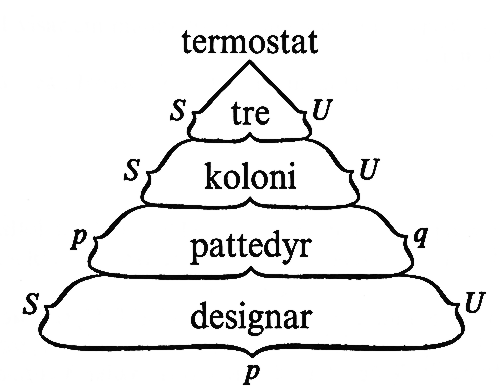
\includegraphics[width=0.5\linewidth]{termostat-designar.png}
\end{center}

\prop{5.13}{a}{Det agenten føretrekkjer å møte, er låg spenning i posisjonen langs aksane modellen dekkjer (3.1).}

\propcont{Å halde målavviket nede er då å følgje gradienten nedover.}

\propcont{Agenten svarar på gradienten slik han når agenten gjennom hinna (5.025), ikkje på forma.\textsuperscript{63,\,64}}

\prop{5.131}{t}{Agenten finn ikkje opp målet, for målet er ein region i eit rom som er gjeve (1.222). Det som er hans, er at han held målet.}

\prop{5.1311}{t}{Mål finst berre mellom to grenser: ein målregion krympa til der agenten alt er, og ein målregion som femner alt mogleg like mykje.}

\propcont{Ein målregion som ikkje skil, er inkje mål, slik eit trykk som inkje tynner ut (2.11), er inkje trykk.}

\prop{5.132}{t}{Der avvik kan rettast når dei kjem, krev navigasjonen berre den lokale gradienten.\textsuperscript{63} Lokale steg gjev global form, utan at nokon ser forma.}

\prop{5.14}{d}{Den \textit{indre spenninga} \msym{σ}\textsubscript{k}(A) er avstanden langs X\textsubscript{k} mellom det agenten møter og målregionen G\textsubscript{k}.}

\propcont{Spenninga i 3.1 ligg over formrommet; den indre ligg i agenten. Det er ho som kan setje politikken i rørsle.}

\prop{5.141}{t}{Indre spenning kjem frå minst to stader: verda mot målregionen, og målet langs éin akse mot målet langs ein annan.}

\propcont{Den første er landskapet (3.1, 5.13), den andre kompromisset (2.13).}

\propcont{Sansinga mot forventinga er noko anna. Det er overrasking, og ho vert målt i prediksjonsavviket (5.11). Ho flyttar modellen. Politikken flyttar ho berre gjennom det den nye modellen predikerer.}

\prop{5.142}{o}{Spenninga i eit stolbein under last, over hinna til ei celle og i eit menneske er same slag storleik, avvik frå ein tilstand som driv ei rørsle attende mot han.}

\propcont{Der ein politikk (5.11) tek imot spenninga, set ho arbeid i gang. I stolbeinet finst ingen politikk.}

\prop{5.143}{t}{Ein agent utan indre spenning langs ein akse har anten nådd målet langs aksen eller mista målet.}

\prop{5.144}{a}{Innanfrå er indre spenning som set arbeid i gang (5.142), kjend som \textit{uro} når målavviket langs aksen står over toleransen. Når det fell under, er ho kjend som \textit{ro}.}

\propcont{Spenning som ikkje set arbeid i gang, vert ikkje kjend. Langs ein akse der ho gjer det, vert eit målavvik modellen predikerer (5.112), kjent som uro før det kjem.}

\propcont{Uro er ikkje overrasking (5.141). (Den som ser sprekken i stolbeinet vekse, er ikkje overraska, men uroleg.)}

\prop{5.1441}{o}{Svolt, smerte og frykt følgjer som regel trugsmål mot det ein organisme må halde. Metting, lindring og tryggleik følgjer at trugsmålet fell bort.}

\prop{5.15}{d}{Evna til å nå same målregion frå ulike utgangspunkt og på ulike vegar er \textit{kompetanse}.}

\prop{5.151}{t}{Kompetansen syner seg berre under forstyrring. Ein kompetent agent når same mål på ein annan veg når vegen vert sperra; ein refleks kjenner berre éin. (Sprekk tappen, kilar stolmakaren beinet fast.)}

\prop{5.152}{d}{Kompetansen kan teljast.}

\propcont{Talet på storleiksordenar av steg politikken sparar samanlikna med blind leiting mot målet G, er\textsuperscript{86}}

\begin{center}\msym{ν}(A;\,G) = log\textsubscript{10}\,(E\,N\textsubscript{blind}(G)\,/\,E\,N\textsubscript{A}(G)),\end{center}

\propcont{med forventingane tekne over utgangspunkt og forstyrringar, og rekna der begge er endelege. \msym{ν} = 0 er inga betring på blind leiting; \msym{ν} < 0 er verre; \msym{ν} > 0 er kompetanse.}

\prop{5.153}{t}{Kvar måling av kompetanse er gjord av ein observatør, i eit rom observatøren har valt (1.321). Målinga seier difor ikkje berre noko om agenten, men òg om observatøren.}

\prop{5.2}{d}{At avvik ikkje er likegyldige for agenten, er \textit{omhug} \msym{ω}(A).\textsuperscript{23,\,68}}

\propcont{For kvar akse X\textsubscript{k} er \msym{ω}\textsubscript{k}(A) kor mykje arbeid ei eining indre spenning langs X\textsubscript{k} set i gang i politikken.}

\propcont{Omhug er ikkje eit tal, men ein profil over aksane.}

\prop{5.201}{t}{Omhug vert målt i arbeid, ikkje i kunnskap eller i hald.}

\propcont{Ein agent kan predikere ein akse fullkome og ikkje røre seg for han, for kunnskap utan omhug predikerer, men endrar ikkje.}

\propcont{Ein agent kan òg arbeide hardt langs ein akse utan å halde han. Om arbeidet held, avgjer politikkane han har og den han vel, ikkje omhugen.}

\propcont{Omhugen set i gang arbeidet, både det som måler og det som endrar.}

\prop{5.21}{d}{\textit{Kapasiteten} \msym{κ}(A) er dei aksane der A, med ein politikk han kan ta i bruk, kan halde målavviket under toleransen (5.11).\textsuperscript{21,\,86}}

\propcont{Der A ikkje har nokon målregion langs aksen, seier kapasiteten kva A kunne halde om han fekk ein.}

\propcont{Kapasiteten er rekna frå eit tidspunkt, og \msym{𝒫}\textsubscript{A} er dei politikkane A enno kan ta i bruk. Når tida for ei handling er forbi, fell dei politikkane som krev henne, ut, og kapasiteten kan krympe.}

\propcont{Kapasiteten er ikkje definert ved prediksjon.}

\prop{5.211}{t}{Prediksjonsavviket og målavviket fastset ikkje kvarandre.}

\propcont{Begge held det møtte (5.11) opp mot noko anna: det eine mot det m ventar, det andre mot det m føretrekkjer.}

\propcont{Ein agent kan difor ha lite D\textsubscript{k} og stort R\textsubscript{k}. Han ser det kome, og det kjem. (Den som høyrer stolbeinet knake og ikkje rekk å reise seg, ser kva som kjem.)}

\propcont{Han kan òg ha stort D\textsubscript{k} og lite R\textsubscript{k}. Han held då aksen ved tilbakekopling, utan å sjå langt. (Den som sit på ein vaklande stol, held balansen ved å rette seg når stolen vippar, ikkje ved å vite når han vil vippe.)}

\prop{5.22}{d}{Det som kan setje agenten i spenning, er den \textit{kognitive lyskjegla} \msym{Γ}(A): aksane der \msym{ω}\textsubscript{k} > 0, kvar med så lang utstrekning fram og attende i tid som måla hans rekk langs han.\textsuperscript{21,\,85,\,90}}

\propcont{Lyskjegla er ikkje grensa for kva agenten sansar eller når, men for kva han har som mål.}

\prop{5.221}{o}{Lyskjegler spenner frå cellulær millisekundrespons til tiårslang konsensus.}

\prop{5.222}{t}{Det som ligg utanfor lyskjegla, finst ikkje \textit{for} agenten, men verkar likevel \textit{på} han.}

\prop{5.223}{t}{Lyskjegla avgjer kva skilnader i formrommet som har noko å seie for agenten.}

\propcont{Innanfor henne møter han ikkje former (5.13), men operasjonane konfigurasjonen tillèt han, \textit{affordansar}.\textsuperscript{12,\,55} (Kroppen møter ikkje forma til stolen, men noko å sitje på.)}

\propcont{Den delen av dei som er felles for heile klassen, er affordansestrukturen i 2.14; det agenten navigerer etter, er resten.}

\prop{5.2231}{t}{Utviding av lyskjegla aktualiserer latente affordansar; innsnevring deaktiverer reelle.\textsuperscript{55,\,70}}

\prop{5.23}{t}{Lyskjegla og kapasiteten er definerte kvar for seg (5.21, 5.22) og treng ikkje falle saman. Ein agent kan bry seg om det han ikkje kan halde, og kunne halde det han ikkje bryr seg om.}

\propcont{Begge er definerte ved strukturen i 5.11 åleine. Dei gjeld difor på kvar grad av agens (5.113), for termostaten like mykje som for stolmakaren.}

\prop{5.231}{d}{Aksane som ligg både i lyskjegla og i kapasiteten, er dei \textit{haldne} aksane: H(A) = \{X\textsubscript{k} \msym{∈} \msym{κ}(A) : \msym{ω}\textsubscript{k}(A) > 0\}.}

\propcont{Langs dei bryr agenten seg og kan halde målavviket under toleransen. Der den faktiske politikken \msym{π}\textsubscript{A} gjer det, viser haldet seg utanfrå som margin: 1 \msym{−} R\textsubscript{k}(\msym{π}\textsubscript{A})\,/\,\msym{ε}.}

\prop{5.232}{d}{Ein akse kan falle utanfor H(A) på tre måtar.}

\propcont{Utan omhug og utan kapasitet: \textit{blindskap}.}

\propcont{Med kapasitet, utan omhug: \textit{likesæle}.}

\propcont{Med omhug, utan kapasitet: \textit{avmakt}.}

\prop{5.2321}{t}{Prediksjonen står på tvers av dei tre.}

\propcont{Dei tre er definerte ved omhug og kapasitet. Omhugen vert ikkje målt i kunnskap (5.201), og kapasiteten er ikkje definert ved prediksjon (5.21, 5.211). Kvar av dei tre kan difor kome med eller utan framsyn.}

\propcont{(Blindskapen er ikkje at ein ikkje ser, men at det ein ser, ikkje set ein i spenning.)}

\propcont{Avmakta kan sjå katastrofen fullkome. Det ho manglar, er ikkje framsyn, men kapasitet.}

\prop{5.2322}{t}{Blindskapen er ikkje nøytral, og det er heller ikkje likesæla eller avmakta, for under alle tre verkar trykka (2.12, 5.222) langs aksen vidare.}

\prop{5.2323}{t}{Gjeve at ein konsekvens langs X\textsubscript{k} viser seg tida \msym{Δ}\textsubscript{k} etter den siste handlinga som kunne hindre han, og at han ikkje kan rettast når han er komen, held A aksen berre om \msym{τ}\textsubscript{k} \msym{≥} \msym{Δ}\textsubscript{k}, eller ved eit hell.}

\propcont{Aksen vert berre halden om konsekvensen vert hindra, og det må skje seinast med den siste handlinga. A vel politikk etter det m predikerer (5.11). Når handlinga må veljast, ligg konsekvensen \msym{Δ}\textsubscript{k} fram, og er \msym{τ}\textsubscript{k} < \msym{Δ}\textsubscript{k}, veit A ikkje då kva som kjem (5.114). Konsekvensen kan då ikkje vere grunnen til valet. Hindrar valet han likevel, er det eit hell.}

\propcont{Det som kan rettast når det kjem, krev ingen slik horisont. (Termostaten held temperaturen utan å sjå fram.)}

\prop{5.2324}{t}{Ligg ein slik akse i lyskjegla, og er \msym{Δ}\textsubscript{k} > \msym{τ}\textsubscript{k}, møter omhugen konsekvensen først når han ikkje kan rettast.}

\propcont{Lyskjegla rekk så langt måla rekk (5.22), og kan difor rekke forbi horisonten. Valet svarar på det A møter og på det m predikerer (5.11, 5.14), og bak horisonten veit A ikkje.}

\propcont{Fanst det ein politikk som ville ha hindra konsekvensen, låg aksen i H(A) (5.231) utan å vere halden, så lenge handlinga kunne takast. Etterpå ligg han utanfor kapasiteten (5.21), medan agenten framleis bryr seg. Det er avmakt (5.232).}

\propcont{Kjem konsekvensen innanfor horisonten etter den siste handlinga, ser agenten han kome utan å kunne hindre han.}

\propcont{Det kallar eg \textit{avmakt i tid}: kapasiteten og framsynet fanst aldri samstundes.}

\prop{5.2325}{t}{Omhugen langs ein akse viser seg under forstyrring.}

\propcont{Forstyrr x\textsubscript{k}. Stig arbeidet i politikken med forstyrringa, ligg aksen i lyskjegla (5.2, 5.22); står arbeidet stilt, ligg han utanfor.}

\propcont{(Set setet ein handbreidd for høgt. Den som bryr seg om setehøgda, tek til å arbeide.)}

\prop{5.2326}{t}{Kapasiteten langs ein akse viser seg når aksen vert gjord til mål.}

\propcont{Gjer aksen til mål for A, ved instruksjon eller insentiv, utan å gje A nye politikkar. Held A då x\textsubscript{k} innanfor målregionen, låg aksen i kapasiteten (5.21).}

\propcont{Held A ikkje aksen sjølv då, er det eit teikn på at han ligg utanfor, men ikkje eit prov. Instruksjonen kan ha vore for veik, eller konsekvensen (5.2323) kan liggje bak horisonten.}

\prop{5.2327}{t}{Prediksjonen langs ein akse viser seg når prognosane vert haldne opp mot det som kjem.}

\propcont{Det gjev D\textsubscript{k} (5.11), og med det horisonten \msym{τ}\textsubscript{k} (5.114). Prediksjonen står på tvers av omhug og kapasitet (5.2321), så prøva er uavhengig av dei to andre.}

\propcont{(Spør stolmakaren kor lenge stolen vil halde, og vent.)}

\prop{5.2328}{t}{Prøvene skil blindskap, likesæle og avmakt frå kvarandre.}

\propcont{Likesæle: inkje svar på forstyrring (5.2325), men hald når aksen vert gjord til mål (5.2326).}

\propcont{Avmakt: arbeidet stig, men x\textsubscript{k} kjem ikkje attende.}

\propcont{Blindskap: inkje svar, og inkje hald sjølv når aksen vert gjord til mål.}

\propcont{Prognosane (5.2327) seier i tillegg om agenten såg avviket kome.}

\propcont{Der skiljet kviler på at aksen ikkje vert halden (5.2326), er det eit teikn, ikkje eit prov.}

\prop{5.233}{t}{I gapet mellom omhug og kapasitet bur strevet.}

\propcont{Gapet er avmakta (5.232). I prøvene (5.2328) viser strevet seg som arbeid som stig, utan at x\textsubscript{k} kjem attende.}

\propcont{Der omhug og kapasitet dekkjer det same, er alt som har noko å seie, innanfor rekkjevidd. Då er det inkje å strekkje seg etter. Trykka kviler ikkje (4.1), så det er framleis noko å halde.}

\prop{5.24}{t}{Omhugen avgjer korleis lyskjegla er fylt: tett langs nokre aksar, tynn langs andre.}

\propcont{Spesialist og generalist er to profilar av same slag. Spesialisten har få høge komponentar, generalisten mange lågare.}

\prop{5.241}{t}{Ein agent med trong omhug kan ha stor kapasitet: mange aksar innanfor rekkjevidd, få som set noko i gang.}

\propcont{Likesæla (5.232) er då ikkje per agent, men per akse.}

\prop{5.25}{t}{Omhugen kan ikkje fyllast ut i ettertid for ei form som alt er navigert. Komponentane måtte vore der då forma vart til. (Kjem omhugen for ryggen først etter at stolen er laga, står han ikkje i stolen.)}

\prop{5.26}{d}{Kor langt eit sjølv rekk, er kor langt lyskjegla rekk.}

\propcont{Hinna seier kvar sjølvet møter verda; lyskjegla seier kva i verda som har noko å seie for sjølvet.}

\propcont{Rekkjevidda krympar, veks og flyttar seg når måla gjer det; hinna kan stå.}

\prop{5.261}{t}{Gjeve 1.2351, er omhug for eit sjølv, sett innanfrå (5.024, 5.144), at noko har noko å seie.}

\propcont{Sett utanfrå er omhug (5.2) kor mykje arbeid avvik set i gang i politikken.}

\prop{5.2611}{t}{Gjeve 1.2351, er det som utanfrå er målavvik over toleransen langs ein akse i lyskjegla, innanfrå uro (5.144).}

\prop{5.2612}{t}{Gjeve 1.2352, er omhug difor ikkje ei kjensle i tillegg til politikken, men at politikken svarar, kjent innanfrå.}

\prop{5.262}{t}{Det som ligg utanfor lyskjegla (5.22), set ikkje arbeid i gang og vert difor ikkje kjent som uro (5.144).}

\propcont{Blindskapen og likesæla er innanfrå inkje, og kan ikkje kjennast att derifrå.}

\prop{5.263}{t}{Grensa for lyskjegla er difor, slik som grensa for tankerommet (1.53), usynleg innanfrå. (Ein kan ikkje kjenne kvar kjensla sluttar.)}

\propcont{Og frå innsida kan inkje system fastslå kva det sjølv kan observere, for ein sjølvmodell som femna si eiga grense, måtte stå utanfor grensa.\textsuperscript{70}}

\propcont{Grensa kan lesast av ein annan, eller i forma.}

\prop{5.27}{d}{Kompetanse i eit rom er \textit{intelligens}: evna til å finne vegar til målregionen, òg vegar som fører bort frå han ei stund og nærare seinare.\textsuperscript{23,\,86,\,91}}

\propcont{Omhug er innhaldet i intelligensen. Omhugen gjev intelligensen noko å gjelde; intelligensen gjev omhugen vegar.}

\prop{5.271}{t}{Kompetansen veks med omhugen berre innanfor kapasiteten, for berre aksar som er haldne, kan navigerast mot målet (5.231), og omhug utover kapasiteten er avmakt (5.232).}

\prop{5.272}{t}{Intelligensen gjeld berre innanfor lyskjegla. Eit problem som ikkje kan setje agenten i spenning, er ikkje \textit{hans} problem.}

\prop{5.3}{t}{Det agenten navigerer i, er det grammatikken (1.62) kan generere.}

\propcont{Agenten tek stega sine med reglar han kjenner og brukar, og den delen av grammatikken er SG. (Ein verkstad som kan dreie, bore og tappe, kan lage stolar av pinnar, men ikkje ein stol støypt i eitt stykke.)}

\prop{5.301}{t}{Grammatikken avgrensar; innanfor det genererbare vektar landskapet (3.1) vegane.}

\prop{5.31}{t}{Av det grammatikken tilbyr, realiserer agenten helst det som minskar spenninga (5.13) langs aksane han held (5.231).}

\propcont{Den venta frie energien som valet av politikk minkar (5.11), har òg eit ledd for uvisse. Agenten kan difor stundom velje det som minskar uvissa, framfor det som minskar spenninga. (Stolmakaren lagar ein prøvestol for å sjå om sambandet held.)}

\prop{5.32}{t}{Sett frå agenten er dei fire operatorane i 1.54 ulike.}

\propcont{C\msym{→}C og K\msym{→}C endrar kva han har tenkt, C\msym{→}K og K\msym{→}K kva han veit (5.118). Det han veit, kan gjere prediksjonen skarpare (5.114).}

\propcont{Men kapasiteten seier kva agenten kan halde (5.21), ikkje kva han veit. Det kjende utvidar kapasiteten berre der det òg gjev han ein politikk som held. Der ein konsekvens kjem for seint til å rettast og må sjåast kome (5.2323), utvidar det kjende ikkje kapasiteten (5.2324), men kan gjere at politikken som held, vert vald.}

\propcont{(Stolmakaren som veit at dampa bøk er sterk nok til eit bøygd bein, kan ikkje lage beinet før ho har ein dampkasse.)}

\propcont{Det tenkte åleine held ingenting.}

\prop{5.4}{d}{Naturlovene (1.2452), slik dei verkar der inkje indre held ei hinne, er \textit{substratet}.}

\propcont{Substratet er grensetilfellet utan agens, utan modell og utan politikk (5.11).}

\propcont{Det legg ned veto mot somme konfigurasjonar og gjev resonans til andre gjennom ufråvikelege avgrensingar.\textsuperscript{26,\,81,\,92,\,93}}

\prop{5.401}{o}{Substratet har to slag parametrar: strukturparametrar (den initiale konfigurasjonen) og funksjonsparametrar (reglane som verkar på konfigurasjonen).\textsuperscript{92}}

\propcont{I dei modellane det er prøvd i, akselererer funksjonsparametrane navigasjonen i formrommet under støy.}

\prop{5.4011}{t}{Strukturparametrane og funksjonsparametrane svarar til startforma og reglane i ein formgrammatikk (1.61).}

\prop{5.402}{t}{Substratet bidreg på to måtar: hardt, ved å leggje ned veto og avgrense kvar landskapet gjeld (1.42), og mjukt, som eitt trykk (2.2) i landskapet.}

\propcont{(Granitt forbyr det bøygde stolbeinet. Bøk tillèt det, men di krappare bogen er, di oftare sprekk emnet.)}

\propcont{Ingen av dei er eit val.}

\prop{5.403}{t}{Substratet har spenning, slik eit stolbein under last har (5.142), men ingen omhug (5.2), for utan politikk set spenninga inkje arbeid i gang.}

\propcont{Det \textit{følgjer} den minste verknaden her og no; det \textit{søkjer} han ikkje. (Stolbeinet som kryp under vekta, følgjer naturlovene. Det prøver ikkje å stå rett.)}

\prop{5.5}{o}{Evna til å navigere hopar seg opp som strukturert informa\-sjon.\textsuperscript{64}}

\propcont{(Handlaget til stolmakaren sit i hendene, i jiggane og i malane.)}

\prop{5.51}{d}{At det ein agent har navigert, utvidar kapasiteten hans, er \textit{læring}.}

\propcont{Det agenten realiserte, står i arkivet (1.41) òg når han har mista det han lærte. Læringa er irreversibel i arkivet, ikkje i kvar agent.}

\prop{5.511}{t}{Summert over agentar flyttar læringa det nærliggande moglege (1.432, 4.4).}

\propcont{Det som vert navigert og realisert, vert busett (1.41) og kjent (1.52), og det busette (1.411) er utgangspunktet for neste steg.}

\prop{5.52}{t}{Læring utvidar \msym{κ}(A), men garanterer ikkje omhug.}

\propcont{Agenten kan lære å halde ein akse han ikkje bryr seg om (5.23). Langs den aksen er det då likesæle (5.232).}

\prop{5.521}{t}{Ei lære som reduserer alle seleksjonstrykk til eitt, verkar sjølv som eit eineveldande trykk (4.5).}

\propcont{Ho pressar landskapet saman til éin dimensjon, slik det tek seg ut for dei som følgjer henne. (Ei lære som seier at ein stol berre skal bere kroppen, ser bort frå prisen, vekta og veret.)}

\propcont{Dei som følgjer henne, realiserer etter det samanpressa landskapet (5.31), og det som endrar kva som vert realisert, er trykk (2.1). Dei andre trykka verkar framleis (2.12).}

\propcont{Langs dei andre aksane er det å følgje læra ikkje rasjonalitet, men systematisk likesæle, og når handlaget er tapt, blindskap (5.232).\textsuperscript{15,\,78}}

\prop{5.5211}{t}{Formene som oppstår under eit samanpressa landskap, er ikkje valde langs dei aksane læra utelèt.}

\propcont{Forma kan då svikte under trykka der (2.12, 5.2322), med mindre arven (4.31) eller materialet ber henne langs aksen.}

\prop{5.5212}{t}{Der læra rår, vert handlaget som svara på dei andre trykka, ikkje lenger øvt.}

\propcont{Det lèt seg ikkje gjenskape frå læra, for éin dimensjon ber ikkje informasjonen til dei andre.}

\propcont{Då krympar kapasiteten (5.21), og handlaget er tapt i agentane (5.51). Det står att i arkivet berre som former. (Handlaget som fletta setet og felte tappen, står att i stolane, ikkje i hendene.)}

\prop{5.53}{t}{Med agentar får landskapet ein ny kanal for endring.}

\propcont{Det kjende går inn i modellane som styrer kva agentane realiserer (5.11, 5.31), og det som endrar sannsynsfordelinga over det som ikkje er forbode, er trykk (2.1).}

\propcont{Det kjende verkar difor sjølv som trykk (1.52, 3.4) på det som kjem etter.}

\prop{5.6}{d}{Den prosessen der eit system held oppe si eiga lyskjegle mot oppløysing over tid, og vidar henne ut der det kan, kallar eg i denne traktaten \textit{liv}.\textsuperscript{85,\,89}}

\propcont{Definisjonen er ikkje biologisk, men stipulert for det teorien treng. Det som er sagt om omhug og kapasitet (5.2, 5.21), kviler ikkje på kva som tel som liv.}

\prop{5.61}{t}{Eit system er levande i den grad det aktivt motverkar at lyskjegla krympar.}

\prop{5.62}{t}{Å halde oppe si eiga lyskjegle krev å halde si eiga hinne.}

\propcont{Utan hinne kjem ingen observasjon inn og inga handling ut (5.02). Og ei hinne som andre held, er ikkje halden av systemet sjølv.}

\propcont{Det levande er difor eit sjølv (5.022), sett utanfrå (5.115).}

\prop{5.63}{d}{Den irreversible kollapsen av lyskjegla til det tomme kallar eg \textit{død}.}

\propcont{Biologisk død er ikkje utleidd av definisjonen. Han er eit korrelat berre under fleire premissar, til dømes at det er hinna til organismen som held måla hans, så lyskjegla fell saman når hinna brest.}

\prop{5.631}{t}{Når lyskjegla er tom, har systemet inkje mål, og det er ikkje lenger ein agent (5.11).}

\propcont{Døden ligg difor på grensa for agentdefinisjonen.}

\prop{5.632}{t}{Døden er slutten på ei avgrensing.}

\propcont{Systemet held ikkje lenger noko (5.631), heller ikkje hinna si. Det som tek slutt, er sjølvet (5.022).}

\prop{5.6321}{t}{Gjeve 1.24, er døden ikkje slutten på oppleving.}

\propcont{Feltet brest ikkje (1.243). Det som brest, er eit mønster i feltet (1.244).}

\propcont{Kva det avgrensa var for seg sjølv, kan ikkje kjennast utanfrå (1.235). Kva som held fram av det, kan difor ikkje avgjerast her.}

\prop{5.64}{t}{Grensa mellom levande og ikkje-levande går gjennom kor mykje av hinna det indre held sjølv (5.62, 5.0222).}

\propcont{Ho går ikkje mellom to slag stoff. (Treet i stolen var levande; stolen er det ikkje.)}

\propcont{Ho er ikkje ei grense i slag, men i grad.}

\prop{5.6401}{t}{Gjeve 1.24, er grensa heller ikkje ei grense mellom to slag substans, for same felt er på begge sider.\textsuperscript{89}}

\prop{5.641}{a}{Eit system som svarar gjennom ei hinne (5.013, 5.02) som står over tid, kan skildrast som om det indre minimerer variasjonell fri energi.\textsuperscript{89}}

\propcont{Skildringa seier at systemet oppdaterer etter sannsyn, som om det hadde ein modell. Kva det føretrekkjer, og om det held det, er andre storleikar (5.11).}

\propcont{Skildringa skil ikkje det levande frå det livlause. Termostaten minimerer fri energi medan andre held hinna hans (5.116); det levande (5.62) gjer det for å halde si eiga hinne.}

\prop{5.7}{a}{\textit{Kjernelikninga.}\textsuperscript{11,\,17,\,21} Forma er grammatikken sin respons på gradienten i landskapet slik agenten estimerer det, projisert på det han kan halde og vekta med omhugen hans:}

\begin{center}\small
\begin{tabular*}{\linewidth}{@{\extracolsep{\fill}}lp{23mm}@{}}
\toprule
Form = SG(\,\msym{ω}(A) \msym{⊙} \msym{∇}\textsubscript{\msym{κ}(A)}\,\(\hat{\Lambda}_A\)(x,\,t)\,) & Grammatikk, landskap, lyskjegle \\
\bottomrule
\end{tabular*}
\end{center}

\propcont{Her er \(\hat{\Lambda}_A\) landskapet slik modellen til A ber det (5.13), ikkje det verkelege landskapet \msym{Λ}.}

\propcont{\msym{∇}\textsubscript{\msym{κ}(A)} er gradienten projisert på kapasiteten (5.21), dei aksane agenten kan halde, ikkje dei han kan predikere. \msym{ω}(A) \msym{⊙} vektar kvar komponent med omhugen, og utanfor lyskjegla er \msym{ω}\textsubscript{k} = 0.}

\propcont{Vektorfeltet kan då vere ulikt null berre langs dei haldne aksane, H(A) (5.231).}

\propcont{Vektorfeltet er gradienten til ein storleik når spenninga lèt seg dele akse for akse. Då er \msym{ω}(A) \msym{⊙} \msym{∇}\textsubscript{\msym{κ}(A)}\(\hat{\Lambda}_A\) = \msym{∇}\,\msym{Σ}\textsubscript{k \msym{∈} H(A)}\,\msym{ω}\textsubscript{k}\,\(\hat{\Lambda}_{A,k}\)(x\textsubscript{k}).}

\propcont{SG(f) er dei formene grammatikken kjem fram til når rørsla følgjer vektorfeltet f nedover. SG(0) = L(SG).}

\prop{5.71}{d}{Likninga er eit strukturelt skjema.}

\propcont{Ho namngjev komponentane, men spesifiserer ikkje den funksjonelle forma til \msym{Λ}, kva reglar i R som slår til, eller dimensjonaliteten til lyskjegla.}

\propcont{Ho seier kva som verkar saman, ikkje kor mykje.}

\prop{5.72}{t}{\textit{Reduksjon.}\textsuperscript{11,\,17} Likninga kan reduserast til fire grensetilfelle, alt etter kva som vert gjort trivielt:}

\propcont{\textit{(i) Rein formgrammatikk}, når \msym{ω}(A) \msym{⊙} \msym{∇}\textsubscript{\msym{κ}(A)}\(\hat{\Lambda}_A\) \msym{≡} 0: det estimerte landskapet er flatt langs dei haldne aksane, eller agenten held ingenting, H(A) = \msym{∅}. Då er Form = SG(0) = L(SG): heile det genererte språket utan seleksjon.}

\propcont{\textit{(ii) Rein tanke-kunnskapsteori}, når grammatikken ikkje genererer noko utover det partisjonen alt rommar, L(SG) = K\,\msym{∪}\,C, og landskapet berre skil det som er kjent å verke, frå resten: \(\hat{\Lambda}_A\) = \msym{𝟙}\textsubscript{\msym{𝕄}\msym{∖}K\textsuperscript{+}}. Spenninga seier her berre om ein posisjon er kjend å verke. Då vert operasjonane reduserte til partisjonsendringar mellom C og K (1.54).}

\propcont{\textit{(iii) Rein optimering}, når grammatikken er fast, språket eit gjeve parameterrom og agenten held alle aksane i det. Då står det att gradientnavigasjon i eit fiksert rom.}

\propcont{\textit{(iv) Den allvitande agenten}, når lyskjegla og kapasiteten femner alle aksar, \msym{ω}\textsubscript{k} er lik langs kvar, horisonten er uendeleg og estimatet er rett, \(\hat{\Lambda}_A\) = \msym{Λ}. Då fell projeksjonen bort, og forma følgjer heile gradienten.}

\propcont{Allvitande tyder her både at agenten predikerer alt og at han kan halde alt.}

\prop{5.721}{t}{Omsette til formrommet (1.54, 1.61) er formgrammatikken og tanke-kunnskapsteorien difor ikkje konkurrerande rammeverk, men degenererte grensetilfelle av same likning.}

\propcont{Kvart av dei oppstår når minst éin av dei tre komponentane vert triviell. Det same gjeld rein optimering og idealet om den allvitande agenten.}

\propcont{Likninga gjer ikkje rammeverka overflødige, og ho er ikkje ein teori om alt. Det ho legg til, er ein presis mekanisme som bind saman form, agens, omhug og konsekvens.}

\propcont{Forma følgjer berre den delen av gradienten agenten både bryr seg om og kan halde (5.7). Langs resten verkar trykka vidare (5.2322). Der arven eller materialet ikkje ber forma (5.5211), kjem konsekvensane.}

\prop{5.722}{t}{Dei historiske designsituasjonane som er granska, er ikkje degenererte.}

\propcont{(i) fell bort, for i kvar av dei navigerer minst éin agent (5.1) og held minst éin akse (5.11). Langs han skil målregionen (5.1311), så det estimerte landskapet langs aksen er ikkje flatt.}

\propcont{(ii) fell bort, for delane i dei er lekamar, og då finn innleiringa delformer som den valde objektdelinga ikkje gav på førehand (1.611). Grammatikken genererer meir enn det som alt er tenkt eller kjent.}

\propcont{(iii) fell bort, for den historiske grammatikken veks med det kjende (1.62), så språket hans er ikkje eit gjeve parameterrom.}

\propcont{(iv) fell bort, for ingen realisert agent er allvitande (5.7221).}

\propcont{Kvart av rammeverka åleine er difor systematisk utilstrekkeleg for desse situasjonane. Dei manglar ikkje detaljar, men lag.}

\prop{5.7221}{t}{Ingen realisert agent er allvitande, verken i prediksjon eller i kapasitet.}

\propcont{Prediksjonshorisonten hans er endeleg (5.1142). Kapasiteten femner ikkje alle aksar, gjeve at ein agent med ein endeleg modell (5.1141) berre kan halde endeleg mange aksar, òg når dei vert gjorde til mål (5.21). Aksane tek ikkje slutt (1.322).}

\propcont{Grensetilfellet (iv) er ein horisont, ikkje ein stad.}

\prop{5.723}{t}{Ingen av dei tre laga kan takast bort utan at likninga fell saman til eitt av grensetilfella i 5.72.}

\prop{5.7231}{o}{Eg kjenner ikkje eit naudsynt fjerde lag som ikkje kan reduserast til desse tre.}

\propcont{Eit fjerde lag ville vise seg som ein skilnad i form som ingen av dei tre kan forklare. (Det kunne vere to rekkjer stolar frå same verkstad, med same reglar og same materiale, under same trykk, laga av agentar med same estimat av landskapet, same omhug og same kapasitet, som likevel skil seg systematisk.)}

\propcont{Ein slik skilnad ville motprove kjernelikninga (5.7) som skjema for form, men ikkje 5.723, at kvart av dei tre laga trengst.}

\prop{5.724}{t}{Formrommet \msym{𝕄} er ikkje eit lag, men grunnen i modellen.}

\propcont{På fast nivå og med faste objekt avheng det ikkje av kva nokon veit (1.2231). Partisjonen \msym{Π} = (K, C, U) er sporet agentane lèt etter seg i \msym{𝕄} gjennom \msym{Λ} (5.118).}

\propcont{På same vilkår kan skiljet mellom \msym{𝕄} og \msym{Π} ikkje kollapse (1.512), for då ville det moglege avhenge av det kjende.}

\propcont{Femtuppelet (\msym{𝕄}, \msym{Π}, SG, \msym{Λ}, \{A\textsubscript{i}\}) inneheld ikkje meir enn grunnen, dei tre laga og sporet dei lèt etter seg.}

\propcont{Gjeve \msym{𝕄}, er dei tre laga, grammatikken, landskapet og agentane med lyskjeglene sine, primitive. Om dei er nok (5.7231), avgjer ikkje modellen, men formene.}

\flowchapter{6 Forma oppstår i feltet mellom agentar}{forma oppstår i feltet mellom agentar}
\mainprop{6}{t}{Forma oppstår i feltet mellom agentar.}

\prop{6.001}{t}{Ei navigert form har to verkande: den som navigerer henne (5.1), og substratet (5.4), som legg ned veto utan å vere agent.}

\propcont{Andre agentar kjem inn på to vegar. Den realiserte forma vert kjend for dei og går inn i modellane deira (1.52, 5.53). Og det ein agent har omhug for, men ikkje kan halde (5.232), vert berre halde om ein annan held det.}

\propcont{Forma oppstår difor mellom agentar \textit{og} mot substratet.}

\prop{6.002}{d}{Feltet mellom agentane er det dei deler (5.026), det som ligg utanfor kvar hinne.}

\prop{6.0021}{t}{Gjeve 1.24, er sjølva mønster i feltet (5.024), og feltet mellom agentane er det same feltet.}

\prop{6.003}{t}{I feltet mellom agentane har trykka to kjelder: substratet (5.4) og politikkane (5.11) til agentane.}

\propcont{Begge avgrensar forma. Berre den andre kan bere omhug, for utan politikk (5.403) set spenninga inkje arbeid i gang.}

\prop{6.01}{d}{Ein agent som ved å navigere realiserer konfigurasjonar i formrommet, er ein \textit{formgjevar}.}

\propcont{Cella, bia, treet, stolmakaren og ingeniøren er formgjevarar. Det som varierer, er materialet agensen er bygd av, ikkje strukturen.}

\prop{6.02}{d}{Ein agent som verkar inn på modellen til ein annan og har følgjene for han i lyskjegla si, er ein \textit{designar}.}

\propcont{Formelt er A designar for A\msym{′} langs aksen X når to vilkår held. A verkar inn på den generative modellen til A\msym{′} langs X: det A gjer, endrar det A\msym{′} møter langs X, og med det modellen hans (5.11).}

\propcont{Og lyskjegla til A femner spenninga til A\msym{′} langs X: eit avvik hjå A\msym{′} langs X set arbeid i gang hjå A (5.2, 5.22).}

\propcont{Designar er ikkje ein ontologisk kategori, men ein konfigurasjon av verknad og omhug.}

\prop{6.021}{t}{Verknad åleine gjer ingen til designar.}

\propcont{Det første vilkåret i 6.02 er naudsynt, ikkje tilstrekkeleg. Det seier at A verkar på A\msym{′}, ikkje at A bryr seg om korleis det går med A\msym{′}.}

\prop{6.0211}{t}{Verknaden treng ikkje gå attende.}

\propcont{A endrar det A\msym{′} møter langs X, utan at A\msym{′} treng endre noko hjå A, for vilkåra i 6.02 krev ingen verknad den andre vegen. Verknaden kan altså vere asymmetrisk.}

\prop{6.022}{t}{Kriteriet for å vere designar er det same for alle formgjevarane i 6.01.}

\propcont{Cella som skil ut eit signalstoff, verkar på naboen. Ho er designar langs aksen berre om avviket hjå naboen set arbeid i gang hjå henne.}

\propcont{Stolmakaren som lagar eit sete, verkar på kroppen som skal sitje. Ho er designar langs setehøgda berre om eit sete som er for høgt for den andre, set arbeid i gang hjå henne.}

\propcont{Cella som berre regulerer si eiga hinne, er ikkje designar langs nokon akse, for lyskjegla hennar femner ikkje spenninga til nokon annan.}

\propcont{Ingen er designar \textit{simpliciter}. Den som er designar, er det \textit{langs nokre aksar} og ikkje langs andre.}

\prop{6.023}{t}{Skiljet designar/ikkje-designar er parametrisk: kor mange aksar og kor mange andre lyskjegla femner.}

\propcont{Profesjonen sjølv er designar berre langs dei aksane der kriteriet er oppfylt. Kva aksar det er, må han vise for å telje som designar.}

\prop{6.024}{t}{Omhug for ein annan krev ingen ny mekanisme.}

\propcont{Han krev berre at stoda til den andre kjem inn i målregionen, slik at eit avvik der set i gang det same arbeidet som eit avvik i eiga stode (5.14, 5.2). Å sjå den andre er ikkje nok, for kunnskap utan omhug (5.201) endrar ikkje.}

\propcont{Omhugen rekk gjennom hinnene, som observasjon inn og handling ut (5.02, 5.027); hinnene står.}

\prop{6.025}{t}{Gjeve 1.24 og 1.2352, skil hinnene til designaren og den ho formgjev for, ikkje to stoff, men to mønster i same felt.}

\prop{6.026}{t}{Ein agent kan leggje spenninga si over på ein annan ved å omsetje henne til eit teikn den andre handlar på. (Bestillinga på tolv stolar er eit slikt teikn; stolane er svaret.)}

\propcont{Overføringa krev ein felles protokoll. Utan han er teiknet støy.}

\prop{6.027}{t}{Gjeve 6.02 og 5.231: langs dei aksane designaren held, held ho det ho verkar inn på; det ho verkar inn på utan å halde, ber den andre åleine.}

\propcont{Som formgjevar verkar designaren inn på modellane til dei som møter formene hennar (1.52, 5.53). Langs ein akse i H(A) set eit avvik hjå den andre arbeid i gang hjå designaren (5.2, 6.02), og ho har ein politikk som held avviket innanfor toleransen (5.21). Vel ho ein slik politikk (5.11), held ho det ho verkar inn på.}

\propcont{Langs dei andre aksane ho verkar inn på, manglar omhugen eller kapasiteten (5.232), eller politikken ho vel, held ikkje det ho kunne halde (5.112, 5.2324). Avviket vert då verande hjå den andre, anten han kjenner det eller ikkje (5.222).}

\propcont{\textit{Åleine} tyder: utan designaren. Ein tredje kan halde aksen for den andre, men designaren gjer det ikkje.}

\prop{6.0271}{t}{Av 6.027 og asymmetrien i 6.0211 følgjer ansvarsproblemet, ikkje av ein metafysisk asymmetri i valfridom.}

\propcont{Designaren endrar det den andre møter, men verknaden krev ingen veg attende (6.0211). Det den andre ber, når designaren berre langs aksane i lyskjegla hennar, og ho kan svare berre langs dei ho held.}

\propcont{Spørsmålet om ansvar vert då eit spørsmål om aksar: kven som verka, kven som heldt, og kven som ber.}

\prop{6.0272}{t}{Designaren held det den andre møter innanfor sin eigen målregion for han, ikkje innanfor målregionen til den andre.}

\propcont{Omhugen for den andre er at stoda hans kjem inn i målregionen til designaren (6.024), og det ho held, er avviket frå denne regionen (5.14, 5.231). Målregionen til den andre ligg i modellen hans, ikkje i hennar.}

\propcont{Der dei to skil seg, ber den andre skilnaden åleine (6.027). (Stolmakaren held setet der ho meiner kroppen vil ha det. Kroppen som sit, har sin eigen målregion.)}

\prop{6.0273}{t}{Langs ein akse designaren verkar inn på utan å ha han i H(A), fell aksen i blindskap, likesæle eller avmakt hjå henne (5.232). I alle tre ber den andre avviket.}

\propcont{Avmakta lettar ikkje det den andre ber. Arbeidet hjå designaren stig, men avviket hjå den andre står. Det er strevet (5.233), ikkje haldet.}

\prop{6.0274}{i}{Stolmakaren held setehøgda for kroppen som skal sitje i stolen. Ryggen etter ein arbeidsdag held ho ikkje. Ryggverken ber den som sit, åleine.}

\prop{6.1}{o}{Former vert som regel navigerte av fleire agentar som svarar på ulike trykk samstundes.}

\propcont{Der 2.13 held, er forma eit kompromiss (2.131). Er ho eit kompromiss mellom agentar, kallar eg henne eit \textit{polyagentisk kompromiss}.\textsuperscript{66,\,67}}

\propcont{Ho trer fram i skjeringspunktet mellom agentane. (I ein kafestol møtest prisen til den som lagar han, stablinga til den som kjøper han, og kroppen til den som sit.)}

\prop{6.11}{o}{Agens finst på mange skalaer samstundes. I dei levande og sosiale systema som er granska, er ein agent som regel sett saman av agentar og sjølv del av agentar.\textsuperscript{22,\,67,\,85,\,87}}

\propcont{Kvar skala har sin eigen kompetanse og si eiga lyskjegle. Delane samarbeider og konkurrerer, innanfor nivå og mellom nivå. (Stolmakaren er sett saman av celler og er sjølv del av ein verkstad og ein marknad.)}

\prop{6.111}{t}{Heilskapen styrer delane berre gjennom landskapet deira.}

\propcont{Ein del svarar på gradienten slik han når delen gjennom hinna (5.13, 5.025). Heilskapen kan altså ikkje styre delen direkte, men bøye landskapet hans, slik at det lokale fallet (5.132) fører dit heilskapen skal.}

\prop{6.1111}{t}{Ei avgjerd i ein del kan difor sjå ut som rein mekanikk når ein ser nær nok, og som eit mål når ein ser på heilskapen.}

\propcont{Kva skala som er rett, er eit val av analysenivå (1.201).}

\prop{6.112}{t}{Kvart nivå navigerer innanfor si eiga lyskjegle (5.272).\textsuperscript{67} Delane på lågare nivå kan difor fremje mål langs aksar som ligg i lyskjegla til heilskapen (6.111), men ikkje i deira eiga.}

\prop{6.113}{t}{Forklaringa nedanfrå viser kva delane gjer, forklaringa ovanfrå kva dei gjer det \textit{for}.}

\propcont{Reduksjonisme og holisme er difor komplementære. Begge forklarer noko; ingen av dei er nok åleine.\textsuperscript{72}}

\prop{6.114}{t}{Der fleire skalaer navigerer same form, vert grammatikkoperasjonar og realiseringar (1.63) utførte på fleire av dei samstundes. Formproduksjonen er då distribuert C\msym{↔}K-ekspansjon.}

\prop{6.12}{o}{Ein biologisk mekanisme for at mange agentar vert éin, er evolusjonære overgangar i individualitet.\textsuperscript{87}}

\propcont{Vilkåret for overgangane er ikkje symmetrisk samspel, men djup interaksjonsstruktur.}

\prop{6.121}{d}{Interaksjonsstrukturen er \textit{djup} når spenninga vert delt: avviket i den eine vert eit avvik i den andre, utan merke om kven det høyrer til.}

\prop{6.1211}{t}{Då set eit avvik i den eine arbeid i gang (5.2) i dei andre, for det er eit avvik i deira eiga stode.}

\propcont{Verkar cella i kopla vev òg inn på naboen, er ho difor designar (6.02) for han langs den delte aksen.}

\prop{6.1212}{t}{Dei kopla delane er ikkje mindre eigennyttige enn før.}

\propcont{I eit kopla nett kjem skaden ein gjer naboen, attende til ein sjølv (6.121). Det som frå nivået over ser ut som samarbeid, er eigennytte.}

\propcont{Sjølvet dei tener, har vorte større.}

\prop{6.122}{a}{Koplinga har eit optimum.}

\propcont{Er ho for laus, vert delane ikkje eitt. Er ho for tett, vert dei ein graut utan delar.}

\prop{6.1221}{t}{Når koplinga brest, krympar sjølvet til delen, og resten av heilskapen vert omgjevnad for han. Delane kan leve vidare. Det som er borte (5.632), er det ytre sjølvet.}

\prop{6.123}{d}{Når ei samling agentar oppfyller 5.11 som heilskap, er ho \textit{éin agent}.}

\propcont{Det er eit \textit{skalasprang} når heilskapen held det ingen del held: ein akse utanfor lyskjeglene til alle delane, eller ein akse der konsekvensen (5.2323) kjem seinare enn horisonten til kvar av delane rekk.}

\begin{center}
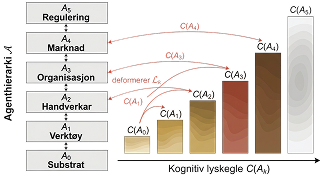
\includegraphics[width=0.9\linewidth]{formgjevarkompetanse/agenthierarki.png}
\end{center}

\prop{6.13}{t}{Agenten vel; landskapet filtrerer.\textsuperscript{66}}

\propcont{Agenten vel blant det grammatikken tilbyr (5.31), og substratet og trykka verkar vidare på det som er valt (6.001, 2.12). Kontrollen er delt.}

\prop{6.131}{o}{I dei systema som er granska, krev utforsking som regel lause koplingar og utnytting tette.}

\prop{6.132}{t}{Kompetente delar jamnar ut landskapet for heilskapen. Der spenninga er delt (6.121), kan ein feil i éin del rettast av dei andre før seleksjonen ser feilen.}

\prop{6.1321}{t}{Ein plan treng difor ikkje vere fullstendig for å verke. Der materialet sperrar vegen (5.402), rettar stolmakaren det teikninga ikkje såg. (Der treet vrir seg, flyttar ho tappen.)}

\prop{6.1322}{t}{Kompetansen i delane kan gje heilskapen tid til å prøve det nye utan å døy av det.}

\prop{6.14}{t}{Designaren er ikkje åleine i landskapet.\textsuperscript{66,\,67,\,93}}

\propcont{Det finst minst éin annan ho verkar inn på (6.02), og som regel fleire som navigerer same form (6.1). Ho navigerer mellom konkurrerande agentar, frå mikrobielt vev til marknadskrefter.}

\propcont{Kompetansen hennar ligg i å samordne uavhengige lyskjegler til ei stabil form.}

\prop{6.2}{o}{Selektiv samanbinding kan etablere globale tilbake\-koplings\-sløyfer.\textsuperscript{66}}

\prop{6.201}{t}{Ei global negativ tilbakekopling som held det ho rettar på (5.113, 6.123), gjer heilskapen til ein agent.}

\prop{6.21}{o}{Hinner ligg i hinner.}

\propcont{Cella held si, vevet si om cellene, organismen si om vevet.}

\prop{6.211}{t}{Når hinnene mellom dei lågare sjølva ber spenninga over (6.121), og ei ny hinne vert halden om alle, kan det oppstå eit sjølv av høgare orden.}

\prop{6.2111}{t}{Gjeve 1.24, vert sjølvet av høgare orden ikkje til ved at opplevingane til dei lågare vert summerte (1.241).}

\propcont{I eitt felt er samansetjing ikkje summering av opplevingar, men endring av grenser.}

\prop{6.22}{t}{Om heilskapen òg vert eit sjølv, avheng av om den nye hinna er sjølvhalden (5.021).}

\prop{6.3}{t}{Utanom agentane har ein \textit{stilart} inga kausal kraft (2.212).\textsuperscript{9,\,15,\,53}}

\propcont{Han er ikkje ei kraft, men eit \textit{mønster\-minne}. Han verkar berre gjennom agentane som kjenner han att: som del av det kjende verkar han som trykk på det neste (5.53), og kanaliserer lyskjeglene deira slik bratte dalveggar kanaliserer formene (3.2).}

\propcont{Det som var aggregat i statistikken (2.211) og sverm i landskapet (3.3), er minne mellom agentane. (Ein standard for setehøgd verkar på same måten, berre gjennom dei som følgjer han.)}

\propcont{Stilarten forenklar navigasjonen ved å tilby eit attkjenneleg tyngdepunkt. Men å formgje «i ein stil» utan å forstå trykka som skapte svermen, er ein kategorifeil.}

\prop{6.31}{o}{For brukaren er stilarten ikkje eit symptom, men eit grensesnitt.\textsuperscript{80}}
\prop{6.311}{t}{Designaren som ignorerer grensesnittet, ignorerer agenten ho formgjev for.\textsuperscript{80}}

\prop{6.312}{t}{Stilen er eit grensesnitt i same meining som persepsjonen er det (5.025, 5.0251): ei koding som viser det brukaren treng for å navigere, ikkje trykka bak. Stilen er kodinga ein kultur deler, persepsjonen kodinga til ein kropp.}

\prop{6.32}{t}{Å navigere med kunnskap om trykka bak stilen, ikkje berre om tyngdepunktet hans, er å representere fleire aksar.}

\propcont{Det vidar modellen. Kapasiteten veks berre der kunnskapen (5.32) òg gjev ein politikk som held.}

\prop{6.4}{t}{Ei ny realisert form utvidar det kjende for dei som ser henne prøvd (1.52), og ho forskyv det nærliggande moglege (1.432, 4.4).\textsuperscript{14,\,79}}

\propcont{Formhistoria tømer ikkje eit lukka repertoar av det kjende, men utvidar det gjennom rørsle.}

\prop{6.5}{t}{Inga form er den siste.}

\propcont{Så lenge agentar navigerer (5.1), vert noko realisert, og landskapet står ikkje stille (4.01). Trykka kviler heller ikkje (4.1). Ein balanse under dei trykka som verka, vert då som regel suboptimal (2.1311) under dei trykka som kjem.\textsuperscript{60,\,61}}

\propcont{Formene er flyktige som balansar. Grammatikkane varer lenger enn formene, men står heller ikkje fast (1.62).}

\propcont{Det som varer, er den generative strukturen: at det finst eit formrom, trykk, eit landskap og agentar.}

\prop{6.51}{t}{Di større lyskjegla (5.22) til ein agent er, di fleire avvik kan setje agenten i spenning.}

\propcont{Så lenge omhugen veks raskare enn kapasiteten, står det att aksar i lyskjegla som agenten ikkje kan halde (5.232). Strevet (5.233) tek då ikkje slutt, og forma han lagar, når ikkje ein sluttilstand.}

\prop{6.511}{t}{Ein agent kan ha som mål å utvide måla sine.}

\propcont{Eit anna mål er ein region i eit gjeve rom (5.131). Når regionen er nådd, står det att å halde regionen.}

\propcont{Målet om å utvide måla flyttar regionen sjølv når han vert nådd. Det har altså ingen sluttilstand, heller ikkje ein å halde.}

\prop{6.5111}{t}{Omhug som vil opne verda, krev meir måling og meir endring enn omhug som vil halde henne slik ho er.}

\propcont{Han legg nye aksar til lyskjegla (6.511), og langs kvar av dei set han i gang arbeid (5.201), både det som måler og det som endrar.}

\prop{6.6}{d}{\textit{Den allmenne forma.} Før realiseringa er det gjeve ei sannsynsfordeling over formrommet.}

\propcont{Det som vert realisert, er éin konfigurasjon x (1.12), og forma hans er strukturen hans (1.212).}

\propcont{\textit{Formmodellen} for x, realisert av agentar \{A\textsubscript{i}\} som navigerer med grammatikken SG, er:\textsuperscript{86,\,89}}

\begin{widebody}
\begin{center}\small
\begin{tabular}{@{}c@{}}
\toprule
\(P(x \mid \{A_i\}, \text{SG}, V) = Z^{-1}\,\mu_{\text{SG}}(x)\,\exp\!\bigl(-\beta \textstyle\sum_i w_i\, \hat{\Lambda}_i(x|_{H(A_i)})\bigr)\) \\
{\footnotesize Eksponentiell vekting} \\[4pt]
\(x \in L(\text{SG}) \setminus V\) \\
{\footnotesize Domenet: det grammatikken kan generere,} \\
{\footnotesize utanom det substratet legg ned veto mot} \\
\bottomrule
\end{tabular}
\end{center}
\end{widebody}

\prop{6.61}{d}{\(\hat{\Lambda}_i(x|_{H(A_i)}) = \sum_{k \in H(A_i)} \omega_k(A_i)\,\hat{\Lambda}_{ik}(x_k)\), der \(\hat{\Lambda}_{ik}\) er det modellen til agent \(i\) predikerer om spenninga i posisjonen langs \(X_k\) (3.1). Kvar agent vurderer berre dei aksane han held, vekta med omhugen sin.}

\propcont{\(w_i \geq 0\) er den relative innverknaden til agenten, med \(\sum_i w_i = 1\).}

\propcont{\(\beta \geq 0\) er seleksjonsstyrken.}

\propcont{\(\mu_{\text{SG}}\) er grunnfordelinga, den fordelinga stega i grammatikken sjølv endar i når inkje vel.}

\prop{6.611}{t}{Det verkelege landskapet \(\Lambda\) står ikkje sjølv i vekta.}

\propcont{Det verkar på fordelinga berre gjennom estimata \(\hat{\Lambda}_i\). Vetoet kjem frå vilkåra, ikkje frå trykka (1.42, 2.1).}

\propcont{Landskapet filtrerer (6.13) etter realiseringa.}

\prop{6.612}{t}{\(\beta = 0\) er nulltrykket; grensa \(\beta \to \infty\) er determinismen, der all masse samlar seg i dei djupaste dalbotnane. Ein grunnare dal får ei vekt som fell eksponentielt med \(\beta\) gonger skilnaden i djupn.}
\prop{6.62}{t}{Av kravet om at \(P\) summerer til éin over \(L(\text{SG}) \setminus V\), følgjer normaliseringskonstanten \(Z\).}

\propcont{Er grunnfordelinga ei sannsynsfordeling og estimata avgrensa nedanfrå, er \(Z\) endeleg; legg grunnfordelinga masse utanfor \(V\), er han positiv.}

\prop{6.63}{t}{Formmodellen sameinar dei tre komponentane frå 5.7: grammatikk (det genererbare \(L(\text{SG})\)), landskap (estimata \(\hat{\Lambda}_{ik}\)) og agentar med lyskjegle og kapasitet (projeksjonen på det dei held, \(H(A_i)\), vekta med \(\omega\)).}

\prop{6.631}{t}{Dei tre komponentane verkar ikkje kvar for seg. Kvar avgrensar den neste.}

\propcont{Grammatikken avgrensar kva som kan genererast.}

\propcont{Det agentane held, avgrensar kva del av landskapet dei svarar på. Resten verkar likevel, men utan at nokon vel.}

\propcont{Estimata av landskapet avgjer kva av det genererbare som er sannsynleg; landskapet sjølv filtrerer (6.611) etterpå.}

\prop{6.632}{t}{At agentane er fleire, er ikkje eit fjerde lag, men same lyskjegle i fleirtal.}

\prop{6.64}{t}{Den allmenne forma er der stega endar; kjernelikninga er steget.}

\propcont{Frå \(x\) føreslår grammatikken eit steg (1.324) til ein nabo \(x'\) med sannsynet \(q(x, x')\). Ligg \(x'\) i \(V\), vert steget avvist; elles vert det godteke med sannsynet \(\min\{1,\, e^{-\beta[\Phi(x')-\Phi(x)]}\}\), der \(\Phi = \sum_i w_i \hat{\Lambda}_i\).}

\propcont{Er straumen i grammatikken like stor kvar veg,}

\begin{center}\(\mu_{\text{SG}}(x)\,q(x,x') = \mu_{\text{SG}}(x')\,q(x',x),\)\end{center}

\propcont{heng \(L(\text{SG}) \setminus V\) saman under stega, står \(\Phi\) stille og er \(Z\) endeleg, så er 6.6 den einaste fordelinga stega kan ende i.}

\propcont{Tida stega treng for å kome dit, er \textit{blandingstida}.}

\prop{6.641}{t}{Når estimata, eller landskapet dei følgjer, endrar seg raskare enn blandingstida, gjeld ikkje fordelinga i 6.6.}

\propcont{Stillstanden er regimet der ho gjeld; bifurkasjonen (4.21) er der ho bryt.}

\prop{6.642}{t}{Med éin agent og \(\beta \to \infty\) går stega aldri oppover.}

\propcont{Langs aksane agenten held, går dei i middel ned langs gradienten til \(\hat{\Lambda}\), til botnen av dalen dei starta i; langs dei andre endrar ikkje \(\Phi\) seg, og stega går fritt etter grunnfordelinga (6.61).}

\propcont{Lèt spenninga seg dele akse for akse, er dette kjernelikninga i skjemaform (5.7).}

\propcont{Tida det tek å kome over ein rygg, veks eksponentielt med \(\beta\) gonger høgda hans, så 6.6 vert ikkje nådd (6.641).}

\propcont{Kva dal det er, avgjer difor historia (4.3), ikkje likninga.}

\prop{6.65}{t}{I formmodellen går grensetilfella i 5.72 att:\textsuperscript{92}}

\propcont{(i) Flatt landskap, \(\beta = 0\) eller \(\hat{\Lambda}_i\) konstant:}

\begin{center}\(P(x) = \mu_{\text{SG}}(x)\,/\,\mu_{\text{SG}}(L(\text{SG}) \setminus V)\) for \(x \notin V\).\end{center}

\propcont{Fordelinga er grammatikken si eiga, avgrensa av vetoet.}

\propcont{(ii) \(L(\text{SG}) = K \cup C\) og \(\hat{\Lambda}_i\) = \msym{𝟙}\textsubscript{\msym{𝕄}\msym{∖}K\textsuperscript{+}}: ei form som er kjend å verke, er \(e^{\beta}\) gonger så sannsynleg som ei anna med same grunnvekt. Seleksjonen verkar berre på grensa mellom dei.}

\propcont{(iii) Fast grammatikk: \(L(\text{SG})\) er eit gjeve parameterrom, og agentane held alle aksane i det. Når \(\beta \to \infty\), står rein gradientnavigasjon i eit fiksert rom att.}

\propcont{(iv) Éin agent som held alle aksar med lik omhug og rett estimat, \(\hat{\Lambda} = \Lambda\), og \(\beta \to \infty\): 6.6 samlar all masse i det globale minimumet av \(\Lambda\) i \(L(\text{SG}) \setminus V\).}

\prop{6.66}{t}{Den allmenne forma viser plassen til formgrammatikken og tanke-kunnskapsteorien: dei er grensetilfelle i henne (6.65). Formlære er difor ikkje eit alternativ til nokon av dei (5.721).}

\propcont{Det formmodellen legg til mekanismen i 5.721, er ei fordeling. Ho seier kor sannsynleg ei form er, gjeve grammatikken, estimata og omhugen, og ho kan haldast opp mot dei formene som vart realiserte.}

\propcont{Påstanden er ikkje at modellen femner alt, men at han kan ta feil.}

\begin{center}
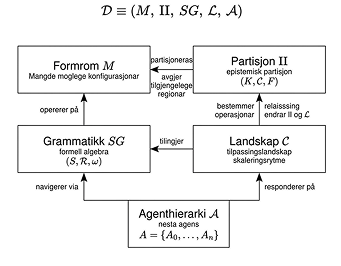
\includegraphics[width=0.92\linewidth]{formgjevarkompetanse/den-generelle-forma.png}
\end{center}

\prop{6.67}{d}{Den \textit{samla omhugen} langs \(X_k\) er \(W_k = \sum_i w_i\,\omega_k(A_i)\), rekna over dei agentane som held aksen.}

\prop{6.671}{t}{Der \(W_k = 0\), vel ingen langs aksen.}

\propcont{Gjeve koordinatane \(x_H\) langs dei haldne aksane, er fordelinga langs aksen grammatikken si eiga, avgrensa til det som ikkje er forbode: \(P(x_k \mid x_H) = \mu_{\text{SG}}(x_k \mid x_H,\, x \notin V)\).}

\propcont{Der er forma berre det moglege, ikkje det valde. Ho fell der ho fell.}

\prop{6.672}{t}{Langs ein akse er variansen nær ein dalbotn omvendt proporsjonal med kor krapp dalen er og kor mykje samla omhug som verkar langs aksen: \(\mathrm{Var}(x_k) \approx 1/(\beta\, W_k\, \hat{\Lambda}''_k)\), der \(\hat{\Lambda}''_k\) er krumminga langs \(X_k\) i dalbotnen. Tilnærminga gjeld når spenninga lèt seg dele akse for akse, agentane er samde om krumminga, grunnfordelinga er flat nær botnen, og det forbodne ikkje ligg nær botnen.}

\propcont{Kanaliseringa (3.2) og omhugen er då to sider av same spreiing.}

\prop{6.673}{t}{Variansen åleine identifiserer ikkje omhugen.}

\propcont{Låg spreiing langs \(X_k\) kan kome av ein stor \(\beta\), av ein krapp dal, av ei trong grunnfordeling \(\mu_{\text{SG}}\) eller av vetoet \(V\), så vel som av ein stor \(W_k\).}

\propcont{I 6.672 står \(\beta\), \(W_k\) og \(\hat{\Lambda}''_k\) som eitt produkt. Variansen seier kor stort produktet er, ikkje kva faktor som ber det.}

\propcont{Utanfor vilkåra i 6.672 kan spreiinga smalne av andre grunnar. Grammatikken og arva malar (4.31) kan gjere grunnfordelinga trong, og materialet skjer bort det forbodne (1.42). Der blandingstida er lang, står arven dessutan att (6.641).}

\propcont{Der \(W_k = 0\), er spreiinga grunnfordelinga si eiga (6.671), og ho kan vere låg likevel.}

\prop{6.674}{t}{Omhugen kan lesast komparativt: gjeve vilkåra nedanfor, kjem ein skilnad i spreiing langs \(X_k\) mellom to formmengder av ein skilnad i \(W_k\).}

\propcont{Vilkåra er at mengdene høyrer til same klasse, med same grammatikk og materiale, altså same \(\mu_{\text{SG}}\) og \(V\); at dei står under same trykk, og at agentane estimerer landskapet langs aksen likt; at \(\beta\) er den same; at begge har nådd fordelinga i 6.6 (6.641); og at grunnfordelinga og vetoet ikkje koplar \(X_k\) til dei andre aksane. Berre agentane er ulike.}

\propcont{Då står \(W_k\) att som det einaste i 6.6 som kan skilje fordelingane langs aksen. Held vilkåra i 6.672 òg, er forholdet mellom variansane det omvende forholdet mellom omhugane:}

\begin{center}\(\mathrm{Var}^{(1)}(x_k)\,/\,\mathrm{Var}^{(2)}(x_k) \approx W_k^{(2)}/W_k^{(1)}.\)\end{center}

\propcont{(To verkstader med same verktøy, same bøk og same kundar lagar stolar. Der setehøgda spreier seg minst, vert ho halden fastast.)}

\propcont{Teoremet kviler på formmodellen. Skil to slike mengder seg systematisk der òg \(W_k\) er lik, viser det eit lag (5.7231) som modellen ikkje har.}

\prop{6.675}{t}{Gjeve at trykket eller målregionen langs \(X_k\) flyttar seg jamt og langsamare enn blandingstida (6.641), og at estimata til dei som held aksen, følgjer med, følgjer ein halden akse etter.}

\propcont{Der \(W_k > 0\), avheng fordelinga langs aksen av estimata (6.61). Ho flyttar seg då med dalbotnen, innan blandingstida (6.64).}

\propcont{Der \(W_k = 0\), avheng ho berre av grunnfordelinga og vetoet (6.671). Aksen følgjer då ikkje, eller berre når grammatikken eller materialet endrar seg. Ein akse låst av arv (4.31) står att til stega har vandra frå han.}

\propcont{Prøva er 5.2325 flytt frå agenten til formene. Ho skil \(W_k > 0\) frå \(W_k = 0\), ikkje stor omhug frå liten.}

\propcont{At aksen ikkje følgjer, er eit teikn, ikkje eit prov. Estimata kan ha stått stille, eller vetoet kan sperre.}

\propcont{Svaret på endring skil omhug frå tvang.}

\prop{6.676}{t}{Forma ber spor av omhug, ikkje bevis for omhug.}

\propcont{Same spor kan kome av omhug, grammatikk, materialtvang, standardisering eller historisk arv (6.673).}

\propcont{Ein standard kan stå i grammatikken, som ein mal i verktøyet, eller i agentane, som eit mønsterminne dei held seg til (6.3). I det første tilfellet er spreiinga grunnfordelinga si. I det andre er ho omhug, men for standarden, ikkje for det standarden ein gong svara på.}

\propcont{Omhugen kan då lesast berre der dei andre kjeldene er haldne like (6.674) eller skilde frå han (6.675).}

\propcont{Ei einskild form gjev ingen av delane, for ho har inga spreiing, og ho har ikkje møtt noka endring.}

\prop{6.6761}{i}{Setehøgda har variert lite over fem hundre år (variasjonskoeffisient 0,07), ornamentet mykje (om lag 1,5).}

\propcont{Den låge spreiinga er eit spor. Ho kan kome av kroppen, men òg av verktøy, standardar og arva malar (6.673).}

\propcont{Prøva er om setehøgda følgjer når kroppane eller bruken endrar seg (6.675). Ei svak form av prøva står alt i arkivet: der bruken er ein annan, er setehøgda det òg. Barkrakken står høgt, stolen i barnehagen lågt.}

\propcont{Om setehøgda følgde då kroppane vart høgare, viser ikkje tala her. Lesinga «kroppen held setehøgda» har stått éi prøve.}

\prop{6.68}{t}{Forma vert vald i det landskapet agentane estimerer langs det dei held, men ho står (6.611) i det landskapet som \textit{er}.}

\prop{6.7}{d}{Ei form \textit{sviktar} langs \(X_k\) når \(x_k\) i bruk kjem inn i ein region der forma ikkje lenger tener funksjonen sin.}

\propcont{Regionen er \textit{sviktregionen} \(F_k\), og grensa hans er \textit{sviktterskelen}. Regionen høyrer til aksen og funksjonen saman, for same verdi kan tene éin funksjon og svikte ein annan.}

\propcont{(Langs styrken til eit stolbein er \(F_k\) dei verdiane der beinet ikkje ber den som set seg.)}

\propcont{Svikt er då ikkje at trykk verkar, men at ein terskel vert kryssa.}

\prop{6.71}{d}{Kor mykje avstanden frå \(x_k\) til \(F_k\) minkar over brukstida \(T\) når ingen held aksen, er \textit{belastninga} \(l_k(T)\).}

\propcont{Belastninga er ikkje eit trykk på fordelinga (2.021), men det som hender med den realiserte forma i bruk. Ho kjem av substratet, som verkar som eit trykk (5.402), til dømes sol og last, og av trykk som flyttar seg (4.1) og tek \(F_k\) med seg. Gjennom belastninga filtrerer det verkelege landskapet (6.611) etter realiseringa.}

\propcont{Eit trykk er \textit{relevant} langs \(X_k\) når det gjev \(l_k(T) > 0\).}

\propcont{(Sola gjer eit stolbein av plast sprøare år for år. Tyngre kroppar flyttar terskelen.)}

\prop{6.72}{d}{Avstanden frå den realiserte \(x_k\) til \(F_k\), før bruken tek til, er den \textit{passive reserven} \(r_k\).}

\propcont{Reserven held utan at nokon handlar. Han kjem av materialet, av redundans, av designarbeid som alt er gjort, og av arv (4.31).}

\propcont{(Eit tjukkare bein står lenger frå \(F_k\). Sprosser mellom beina ber stolen om ein tapp losnar.)}

\propcont{Det som vart halde då forma vart til, står slik att som reserve.}

\prop{6.73}{t}{Gjeve at \(X_k\) er uhalden i bruk, \(W_k = 0\), at eit relevant trykk verkar, \(l_k(T) > 0\), og at reserven er for liten, \(r_k < l_k(T)\), er svikt langs \(X_k\) venta innan \(T\).}

\propcont{Her er \(W_k\) rekna som i 6.67, over dei som verkar på forma medan ho er i bruk.}

\propcont{Med \(W_k = 0\) held ingen aksen i bruk. Avstanden var \(r_k\) (6.72) og minkar då med \(l_k(T)\) (6.71). Når \(l_k(T) > r_k\), kjem \(x_k\) inn i \(F_k\) før \(T\) er ute (6.7).}

\propcont{Svikten er venta, ikkje viss, for \(l_k(T)\) og \(r_k\) er estimat.}

\propcont{Med det første og det andre vilkåret åleine er svikt ikkje venta, for ein uhalden akse kan vere robust gratis, gjennom reserven.}

\propcont{Med det andre og det tredje åleine er svikt heller ikkje venta. Held nokon aksen, kan han føre \(x_k\) attende, så sant estimatet hans er rett (5.231, 6.68).}

\propcont{(Det tredje vilkåret føreset det andre, for reserven er aldri negativ.)}

\propcont{Å vere uhalden er ikkje å svikte.}

\prop{6.74}{d}{Mengda av aksar som er uhaldne i bruk, og der belastninga er større enn reserven, er \textit{det predikerte sviktrommet}:}

\begin{center}\(S(T) = \{X_k : W_k = 0 \text{ i bruk og } l_k(T) > r_k\}.\)\end{center}

\prop{6.741}{t}{Sviktrommet er prediktivt, og det kan motprovast.}

\propcont{Langs kvar akse i \(S(T)\) er svikt venta innan \(T\) (6.73). Utanfor \(S(T)\) er han ikkje venta, for der held anten nokon aksen, eller reserven ber belastninga.}

\propcont{Svikt utanfor \(S(T)\) langs ein akse ingen held, eller inga svikt inne i \(S(T)\), motprovar då anten modellen eller estimata han vart brukt med. Svikt langs ein akse nokon held, kan òg kome av at estimatet til den som held, var galt (6.68).}

\propcont{Estimata er tre. Kven som held aksen, lèt seg prøve på agentane (5.2328) og lesast av formene (6.674, 6.675). Belastninga og reserven kviler på det som er prøvd (1.52).}

\prop{6.742}{d}{Kva av blindskap, likesæle og avmakt (5.232) ein akse i \(S(T)\) fell i hjå ein agent, er \textit{sviktsignaturen} langs aksen for den agenten.}

\propcont{Ingen held aksen, så han fell utanfor for kvar agent som verkar på forma, på ein av dei tre måtane.}

\propcont{Om signaturen er relevant for ein agent, er ikkje eit spørsmål modellen svarar på, men eit spørsmål agenten stiller når han les modellen.}

\prop{6.75}{d}{Kor mange horisontar ein svikt ligg fram, er \textit{sviktlatensen}: \(\rho_k(A) = \Delta_k/\tau_k(A)\).}

\propcont{\(\Delta_k\) er tida frå den siste handlinga som kunne hindre svikten, til han kjem (5.2323). \(\tau_k(A)\) er horisonten til A langs aksen (5.114). Er horisonten null, er \(\rho_k(A)\) uendeleg.}

\propcont{Definisjonen gjeld på same måten for kvar konsekvens langs \(X_k\) som ikkje kan rettast når han er komen.}

\needspace{12\baselineskip}
\prop{6.751}{d}{Grensa \(\rho_k = 1\) deler svikten i tre regime:}

\nopagebreak
\begin{widebody}
\begin{center}\small
\begin{tabular*}{\linewidth}{@{\extracolsep{\fill}}lp{61mm}@{}}
\toprule
\(\rho_k(A) \le 1\) & \textit{Innanfrå}: horisonten til A rekk fram til svikten frå den siste handlinga som kunne hindre han. \\[3pt]
\(\rho_k(A) > 1,\ \tau'_k \ge \Delta_k\) & \textit{Leseleg utanfrå}: A ser ikkje svikten kome, men ein representasjon A har tilgang til, rekk fram. \\[3pt]
\(\rho_k(A) > 1,\ \tau'_k < \Delta_k\) & \textit{Strukturelt usynleg}: ingen representasjon A har tilgang til, rekk fram. \\
\bottomrule
\end{tabular*}
\end{center}
\end{widebody}

\propcont{Her er \(\tau'_k\) den lengste horisonten langs \(X_k\) blant dei representasjonane A har tilgang til utanom sin eigen modell: andre agentar, simuleringar, standardar, kollektivt minne og vitskap.}

\propcont{Regimet er relativt til den som les. Ein svikt som er usynleg for den som formgav, kan vere leseleg (1.531) for ein med aksen i lyskjegla si og ein lengre horisont. Det som er strukturelt usynleg i dag, kan bli leseleg når ein ny representasjon kjem til.}

\prop{6.7511}{t}{Grensa \(\rho_k = 1\) er den einaste prinsipielle grensa på sviktlatensen.}

\propcont{Ved \(\rho_k = 1\) rekk horisonten akkurat fram til svikten frå den siste handlinga som kunne hindre han. Under grensa kan A sjå svikten kome medan han enno kan hindrast (5.2323); over grensa kan A det ikkje.}

\propcont{Ei grense ved 0,1 eller ved 100 markerer ingen slik skilnad. Ho gjev ein tryggleiksmargin eller ein storleiksorden, og begge er avtalar.}

\propcont{Grensa mellom det leselege og det usynlege ligg ikkje i \(\rho_k\), men i om ein annan representasjon rekk fram. Ho kan altså ikkje vere eit tal på \(\rho_k\).}

\prop{6.752}{t}{Ein svikt langt fram kan liggje innanfrå.}

\propcont{Stor \(\Delta_k\) gjev ikkje stor \(\rho_k\) når horisonten langs aksen er like lang. (Ein tapp av rått tre krympar når treet tørkar, og sambandet losnar etter ein vinter. Stolmakaren veit det før ho set tappen inn.)}

\propcont{Det er ikkje tida åleine som avgjer om svikten ligg innanfrå, men forholdet.}

\prop{6.753}{t}{Ein svikt like framme kan liggje bak horisonten.}

\propcont{Liten \(\Delta_k\) gjev stor \(\rho_k\) når horisonten er endå mindre. (Ein kvist inne i eit stolbein kan få beinet til å knekke første gongen nokon set seg tungt. Den som ser beinet utanfrå, har ingen horisont langs styrken til nettopp det beinet.)}

\prop{6.754}{t}{Ei simulering forlengjer horisonten gjennom ein representasjon.}

\propcont{Ei utrekning eller ei lastprøve på andre bein av same slag (1.52) kan vise kva beinet toler etter mange tusen sitjingar, før stolen er laga.}

\propcont{Tek A resultatet inn i modellen sin, veks \(\tau_k(A)\), og svikten flyttar seg frå det leselege utanfrå til det A ser innanfrå (6.751).}

\prop{6.755}{t}{Kollektivt minne og standardar er ein lånt horisont.}

\propcont{Ein standard for kor sterkt eit stolbein skal vere, ber erfaringa frå mange stolar som har svikta. Standarden rekk lenger fram enn den som følgjer han.}

\propcont{For den som følgjer standarden utan å kjenne grunnen, er \(\rho_k > 1\), men svikten er leseleg utanfrå (6.751).}

\propcont{Den som følgjer standarden, kan hindre svikten utan å sjå han kome. Sett frå han er det eit hell (5.2323); sett frå standarden er det framsyn.}

\prop{6.756}{i}{Ergonomi: prøvesitjinga ser ein time fram, og ryggverken kjem etter ein arbeidsdag. For den som prøvesit, er \(\rho \approx 8\). Ergonomien og erfaringa til dei som har sete ein arbeidsdag, rekk fram, så svikten er leseleg utanfrå.}

\propcont{Eingongskoppen: bruken ser tjue minutt fram, og nedbrytinga tek fire hundre år, så \(\rho \sim 10^7\). Kjemien rekk likevel fire hundre år fram, og nedbrytinga er leseleg utanfrå. For den som drikk, ligg ho bak horisonten.}

\propcont{Forholdstala skil seg med seks storleiksordenar, og regimet er det same.}

\prop{6.76}{t}{Sviktlatensen seier om svikten kan sjåast kome, ikkje om han kan hindrast.}

\propcont{Å sjå er prediksjon (5.114), å hindre er kapasitet (5.21), og den eine fastset ikkje den andre (5.211).}

\propcont{Blindskapen ser ikkje etter. Aksen set ikkje agenten i spenning, og då set han heller ikkje i gang det arbeidet som måler (5.201, 5.262). Med \(\rho_k \le 1\) ser han likevel svikten kome (5.2321).}

\propcont{Avmakta kan sjå svikten kome når \(\rho_k \le 1\) (5.2321), og med \(\rho_k > 1\) seinare, når han ikkje lenger kan hindrast (5.2324). Ho kjenner han som uro før han kjem og når han kjem (5.144), men kan ikkje halde aksen.}

\propcont{Likesæla kunne halde aksen og sjå etter svikten. Ho gjer ingen av delane, for aksen set ikkje arbeid i gang (5.201, 5.262). Med \(\rho_k \le 1\) ser ho likevel svikten kome (5.2321).}

\propcont{Kven som kunne sjå, og kven som kunne hindre, er to spørsmål.}

\prop{6.77}{t}{Gjeve 6.73 og 6.74, kan ein teori som ikkje skil haldne frå uhaldne aksar og ikkje kjenner reserven, ikkje peike ut \(S(T)\) før svikten.\textsuperscript{21,\,70}}

\propcont{\(S(T)\) er gjeve ved \(W_k\), \(l_k(T)\) og \(r_k\). Utan skiljet veit teorien ikkje kvar \(W_k = 0\). Utan reserven veit han ikkje kvar \(l_k(T) > r_k\).}

\propcont{Ein slik teori kan berre registrere svikten i ettertid.}

\propcont{Prediksjonen krev likevel ikkje eit ferdig kart over landskapet, for landskapet lèt seg berre lodde i ettertid (3.11). Han krev dei tre lokale estimata i 6.741.}

\prop{6.771}{t}{Den predikerte svikten kjem i former grammatikken kunne generere, langs aksar ingen held (6.74), under trykk i det verkelege landskapet (6.68).}

\propcont{Grammatikken åleine (5.72 i) veit kva som \textit{kan} bli, ikkje kva som \textit{vil} svikte.}

\propcont{Tanke-kunnskapsteorien åleine (5.72 ii) veit kva som er kjent, ikkje kvar det ukjende vil slå til.}

\propcont{Optimeringa åleine (5.72 iii) skjerper dei aksane ho har, og er blind for resten.}

\propcont{Prediksjonen krev difor alle tre laga som omgrep.}

\prop{6.7711}{t}{For den allvitande agenten (5.72 iv) ville \(S(T)\) vere tom same kva reserven var, for han held kvar akse.}

\propcont{Det som stod att, ville vere kompromisset sjølv, der 2.13 held (2.131).}

\propcont{Men grensetilfellet (iv) er ein horisont (5.7221), ikkje ein stad.}

\prop{6.772}{t}{Å forklare ei form er å forklare kvifor dei andre ikkje vart realiserte (1.131). Langs aksar ingen heldt (6.671), vart dei ikkje utelukka av noko val.}

\propcont{Ein teori som ikkje skil desse aksane frå dei andre, kan ikkje peike ut \(S(T)\) (6.77). Han forklarer ikkje form, men katalogiserer henne.}

\propcont{Sviktrommet er såleis ikkje ein empirisk bonus, men prøvesteinen på at teorien forklarer form.}

\prop{6.8}{i}{Monoblokkstolen er ein hagestol sprøytestøypt i eitt stykke polypropylen.}

\propcont{Stolen er dømet som går heile vegen: formrom, grammatikk, trykk, agentar, omhug og kapasitet, predikert uhalden akse, faktisk svikt og det arkivet (1.41) viser.}

\prop{6.81}{i}{Klassen er stolar (1.3), og objekta på det valde nivået er sete, rygg og bein (1.2).}

\propcont{I monoblokkstolen er dei ikkje skilde lekamar, men delformer i éin lekam (1.611).}

\propcont{Aksane (1.32) som tel her, er setehøgda, tjukkleiken på veggane, kor mykje beina vidar seg ut, kor mykje UV-stabilisator plasten har, og kor sterke beina og ryggen er etter år i sol. Den siste aksen kallar eg \(X_s\).}

\prop{6.82}{o}{Grammatikken er sprøytestøypinga.}

\propcont{Forma må sleppe verktøyet, så flatene som går i opningsretninga, har slipp, ein liten vinkel. Veggane må vere om lag like tjukke, elles fyller plasten verktøyet ujamt og kjølnar ujamt.}

\propcont{Stablinga krev bein som vidar seg ut nedover, så den eine stolen går ned i den andre.}

\prop{6.83}{o}{Trykka er prisen per stol, stablinga, vekta til stolen, kroppen og veret.}

\propcont{Prisen er for det meste plasten, og han dreg veggane tynnare. Kroppen som sit, dreg dei tjukkare. Sola og kulda gjer plasten sprø.}

\propcont{Langs tjukkleiken på veggane strir altså prisen og kroppen.}

\prop{6.84}{i}{Fire verkande står om stolen.}

\propcont{Produsenten held materialkostnaden og stablinga. Kafeeigaren, som kjøper, held prisen og stablinga. Gjesten held komforten i dei minutta han sit.}

\propcont{Substratet (5.4) er polypropylenet, slik naturlovene verkar på det. Det vert sprøtt i sollys og kryp under last, og det er ikkje agent.}

\prop{6.85}{t}{Gjeve premissane i 6.851 til 6.853, held ingen av dei tre agentane \(X_s\), og hjå kvar fell aksen utanfor (5.232) på sin eigen måte.}

\prop{6.851}{t}{Gjeve at produsenten held \(X_s\) når aksen vert gjord til mål, og at stolen hans ikkje vert endra når han får vite at stolane sviktar i sol, er \(X_s\) likesæle hjå produsenten.}

\propcont{Det første premisset gjev kapasitet (5.2326). Stabilisator og tjukkare bein ligg innanfor grammatikken (6.82). (Krev ein kjøpar at stolen skal tole sol, kan produsenten levere han.)}

\propcont{Det andre gjev at omhugen manglar (5.2325), for forstyrringa set ikkje arbeid i gang. Kapasitet utan omhug er likesæle (5.232).}

\propcont{Svarar produsenten, men svakt, ligg aksen i lyskjegla hans med liten omhug. Då er svikten eit kompromiss med prisen der 2.13 held (2.131), ikkje likesæle.}

\prop{6.852}{t}{Gjeve at gjesten sit i minutt, ikkje rår over stolen og ikkje set i gang arbeid når stolen vert eldre, er \(X_s\) blindskap hjå han.}

\propcont{Aldringa set ikkje arbeid i gang hjå han, så aksen ligg utanfor lyskjegla (5.22, 5.2325). (Måla hans rekk ikkje år fram.) Og han har ingen politikk som held styrken til ein stol han ikkje rår over (5.21).}

\propcont{Utan omhug og utan kapasitet er det blindskap (5.232).}

\prop{6.853}{t}{Gjeve at kafeeigaren ser stolane eldast, men ikkje kan byte materialet eller skjerme stolane for sola, er \(X_s\) avmakt hjå han, med framsyn.}

\propcont{Plasten bleiknar og sprekk i overflata, og arbeidet hans stig: han ser etter, flyttar stolar og vurderer (5.2325). Men ingen politikk han har, fører styrken attende (5.2326). Omhug utan kapasitet er avmakt (5.232).}

\propcont{Fanst det ein stabilisert stol å kjøpe då han kjøpte, hadde han kapasitet, men horisonten hans rakk ikkje år fram. No har han framsyn, men ikkje kapasitet. Dei to fanst ikkje samstundes, og det er avmakt i tid (5.2324).}

\prop{6.86}{t}{Gjeve 6.85 og at reserven ikkje ber nokre år i sol, ligg \(X_s\) i det predikerte sviktrommet \(S(T)\) (6.74) for ei brukstid \(T\) på nokre år.}

\propcont{Ingen av dei tre held aksen (6.85), og produsenten verkar ikkje på stolen i bruk. Altså er \(W_s = 0\) i bruk (6.67).}

\propcont{Belastninga kjem av sola og sitjinga og veks med åra, så \(l_s(T) > 0\) (6.71).}

\propcont{Reserven er liten, for beina er tynne (6.72), og lite stabilisator gjer belastninga frå sola stor. Estimatet er at reserven ikkje ber nokre år i sol, \(r_s < l_s(T)\).}

\propcont{Etter 6.73 er svikt langs \(X_s\) då venta innan \(T\).}

\prop{6.87}{t}{Har produsenten data om aldringa til plasten i sol, er sviktlatensen langs \(X_s\) ulik for kjøparen og produsenten (6.75).}

\propcont{Den siste handlinga som kunne hindre svikten, er valet av plast og veggar, eller valet av stol. Svikten kjem år etter.}

\propcont{Kjøparen prøvesit i minutt, og horisonten hans langs \(X_s\) er minutt. For han er \(\rho_s \gg 1\). Har han tilgang til slike data, er svikten likevel leseleg utanfrå (6.751).}

\propcont{Har produsenten slike data, er horisonten hans år. For han er då \(\rho_s \le 1\), og svikten ligg innanfrå.}

\propcont{Med slike data ser produsenten altså svikten kome og held ikkje aksen. Kjøparen kunne ha valt ein annan stol, men såg ikkje svikten kome då han valde (6.853). Framsynet (5.2321) står på tvers av haldet.}

\prop{6.88}{o}{Monoblokkstolar som har stått i sol i fleire år, vert sprø og kan brekke under last, i beina eller i ryggen.}

\propcont{Det vert òg laga monoblokkstolar med UV-stabilisator, og dei vert som regel sprø mykje seinare i sol.}

\prop{6.89}{t}{Gjeve 6.86 og premissane i 6.851, ber brotet sviktsignaturen (6.742) til likesæle hjå den som laga stolen, ikkje til blindskap.}

\propcont{Blindskap krev at kapasiteten mangla (5.232). Kapasiteten fanst, for stolar av same klasse med stabilisator vert laga (6.88), og produsenten held aksen når han vert gjord til mål (6.851).}

\propcont{Prøva er den komparative (6.674), brukt på svikt i staden for på spreiing: same klasse, same grammatikk, same bruk og same sol, ulikt berre i stabilisatoren og veggane. Stolen med stabilisator sviktar mykje seinare (6.88). Skilnaden ligg då i det som vart gjort då stolen vart til, ikkje i klassen eller bruken.}

\propcont{At monoblokkstolane liknar kvarandre, er eit anna spor, og det er ikkje eit spor av omhug åleine, for grammatikken gjer grunnfordelinga trong (6.82, 6.673).}

\propcont{Dømet kan motprovast (6.741). Held stolar utan stabilisator og med tynne bein seg i sol år etter år, er estimata gale. Sviktar stabiliserte stolar like tidleg, ligg skilnaden ikkje i haldet.}

\propcont{Lesen mot den stabiliserte, viser den brotne stolen kva som vart halde, og kvar haldet slutta.}

\flowchapter{7 Forma er eit arkiv over kva som vart halde}{forma er eit arkiv over kva som vart halde}
\mainprop{7}{t}{Forma er eit arkiv over kva som vart halde.}

\prop{7.01}{t}{Langs dei aksane nokon heldt, er forma vald; langs dei andre fell ho.}

\propcont{Der \(W_k > 0\), vektar estimata posisjonane langs aksen (6.61, 6.67); der \(W_k = 0\), fell forma der grammatikken og substratet lèt henne falle (6.671).}

\propcont{Gjeve at ei form vert navigert av endeleg mange agentar, og at kvar av dei held endeleg mange aksar (5.7221), er ho vald langs endeleg mange. Ho er likevel eksakt langs alle (1.12, 1.32), og aksane tek ikkje slutt (1.322).}

\propcont{Forma rekk difor lenger enn haldet.}

\prop{7.011}{t}{Omhug utan kapasitet når ikkje fram til forma.}

\propcont{I formmodellen vel kvar agent berre langs dei aksane han held (6.61), og den samla omhugen er rekna over dei som held aksen (6.67).}

\propcont{Der ingen held aksen, er \(W_k = 0\), same om det manglar omhug, kapasitet eller begge (5.232). Forma fell då likt (6.671), og i formmodellen set strevet i avmakta (5.233) ikkje spor langs aksen.}

\propcont{Arkivet viser kvar haldet slutta, ikkje kvifor.}

\prop{7.02}{t}{Gjeve 1.2351 og 5.261, er forma, langs dei haldne aksane (7.01), omhug, sett utanfrå.}

\propcont{Den som avviser modulen (1.25), mistar lesinga, men ikkje arkivet.}

\prop{7.03}{t}{Gjenstanden er eit arkiv. Han ber omhug som ingen lenger held.}

\propcont{Som steinen held han ikkje si eiga hinne (5.023), og som setet er han ingen agent (5.113). Det han viser langs dei haldne aksane, sette andre der (7.01). Omhugen han ber, er lånt: omhugen til dei som forma han, festa i materialet.}

\propcont{Ein laga gjenstand er slik ei avleiring av kva nokon heldt og ikkje heldt.}

\propcont{Den lånte omhugen står att som reserve (6.72). Held ingen aksen i bruk, og er belastninga større enn reserven, er svikt venta (6.73). (Monoblokkstolen i 6.86 fekk ingen lånt omhug med seg langs styrken i sol.)}

\propcont{Belastninga tærer på den lånte omhugen.}

\prop{7.1}{t}{Arkivet ber spor av kva som vart halde, ikkje bevis.}

\propcont{Sporet er ikkje tilfeldig, for skiljet mellom det valde og det uvalde følgjer grensa for det agentane heldt (7.01).}

\propcont{Men same spor kan kome av grammatikk, materialtvang, standardisering eller arv (6.676). Haldet kan lesast der dei andre kjeldene er dei same (6.674), eller der aksen følgjer når trykket eller målregionen flyttar seg (6.675).}

\propcont{Det uhaldne kan lesast i svikten (6.741). Ein svikt viser anten at ingen heldt aksen i bruk og reserven var for liten, eller at modellen eller estimata tok feil.}

\propcont{Kvar av dei tre lesingane er ein skilnad: mellom to formmengder, mellom før og etter, mellom det venta og det som kom.}

\propcont{Forma er ei ordning av skilnader (1), og arkivet hennar vert lese i skilnader.}

\prop{7.11}{t}{Former for same funksjon, laga under ulikt hald, kan lesast mot kvarandre.}

\propcont{Vart aksen halden i éi av formene, låg haldet innanfor grammatikken og materialet (5.3). Der han ikkje vart halden i ei anna under vilkåra i 6.674, mangla det då omhug eller kapasitet. Kva av dei som mangla, viser prøvene på agentane (5.2328).}

\propcont{Det den eine heldt, er målestokken for det den andre ikkje heldt.}

\prop{7.12}{t}{Arkivet er ikkje ei skulding, men eit faktum.}

\propcont{Den brotne stolen i 6.89 er tilfelle (1.1). Likesæla brotet ber under premissane i 6.851, er ein sviktsignatur (6.742), ein stad i arkivet og ikkje ein dom over den som laga stolen. (Same faktumet som gjer geologi leseleg, gjer design leseleg.\textsuperscript{72})}

\prop{7.2}{t}{Arkivet over haldet er òg eit arkiv over kven som ber.}

\propcont{Designhandlinga verkar inn på modellane til andre, og forma står att når handlinga er over (7.03). Det designaren verkar inn på utan å halde, ber den andre åleine (6.027).}

\propcont{Der aksen vart halden, viser arkivet difor eit hald. Der forma rører den andre langs ein akse ingen heldt, viser det ein som ber åleine.}

\propcont{Òg langs dei haldne aksane står målregionen til designaren i forma (6.0272), og den andre ber skilnaden mot sin eigen.}

\propcont{Så langt arkivet kan lesast (7.1), står ansvaret (6.0271) i forma.}

\prop{7.21}{t}{Det ingen heldt, ventar i forma på den som kjem etter.}

\propcont{Den som seinare møter forma (7.03), ber avviket utan dei som forma henne (6.027), anten han kjenner det eller ikkje (5.222). (Gjesten veit inkje før beinet brest.)}

\propcont{Har han aksen i lyskjegla si og kan ikkje halde aksen, er det avmakt hjå han (5.232), og avviket over toleransen er kjent som uro (5.144).}

\propcont{Uroa er hjå den som ikkje var med langs aksen då forma vart vald.}

\prop{7.22}{t}{Modellen seier ikkje kva som bør haldast.}

\propcont{Han måler arbeid (5.201) og hald (5.231), og han viser kven som ber det ingen held (7.21). Målregionane høyrer til agentane (5.11), og modellen legg ingen eigen til.}

\propcont{Kva som følgjer av det han viser, avheng av omhugen til den som les, for kunnskap utan omhug endrar ikkje (5.201).}

\propcont{Modellen dømer ikkje, men skildrar.}

\prop{7.23}{t}{Omhugen veit ikkje sjølv kor langt han rakk.}

\propcont{Grensa for lyskjegla er usynleg innanfrå (5.263). Kvar haldet slutta i blindskap eller likesæle, kan designaren difor ikkje kjenne att derifrå (5.262), sjølv når ho ser svikten kome (5.2321, 6.76).}

\propcont{Sløyfa vert lukka utanfrå: av svaret frå den som tok imot, eller av ein annan som les forma (6.751). Modellen kan vere ein slik annan.}

\propcont{Å vise kven som ber, er nok til å gjere ansvaret synleg.}

\prop{7.3}{t}{Arkivet kan villeie.}

\propcont{Fire motdøme (7.31 til 7.34) viser kvar teorien nesten brest, kva som bergar han, og kva det kostar.}

\prop{7.31}{t}{Ei velgjord form frå likesæle hender kan sjå halden ut.}

\propcont{Ein stolmakar som ikkje bryr seg om styrken i beina, har berre tjukk eik, og stolen står i hundre år.}

\propcont{Reserven var stor og kosta ingen omhug (6.72). Den som les stolen åleine, les eit hald som ikkje var.}

\propcont{Teorien vert berga av reserven og av prøva på svar. Byter stolmakaren til furu, kjem ikkje styrken attende, for beina vert ikkje tjukkare (6.675).}

\propcont{Utan ei slik endring, og utan ein annan stolmakar med same eik og ein annan omhug (6.674), kan teorien ikkje skilje haldet frå hellet.}

\propcont{Om den eine stolen må han teie.}

\prop{7.32}{t}{Den som ser svikten kome og ikkje kan hindre han, ser ut som den blinde.}

\propcont{Kafeeigaren i 6.853 ser stolane eldast og veit kva som kjem. Han bryr seg, men kan ikkje halde styrken.}

\propcont{Var avmakt å ikkje sjå svikten kome, passa han i ingen av dei tre (5.232). Teorien braut her så lenge prediksjon og kapasitet gjekk i eitt.}

\propcont{Skiljet i 5.211 bergar teorien. Avmakta manglar ikkje framsyn (5.2321), men kapasitet.}

\propcont{Men framsynet står ikkje i forma. Svikten kjem same om kafeeigaren ser han kome eller ikkje (6.73), og strevet hans set ikkje spor langs aksen (7.011). Om nokon såg, viser prognosane (5.2327), ikkje brotet.}

\propcont{Arkivet tek vare på haldet, ikkje på framsynet.}

\prop{7.33}{t}{Arkivet kan vise ei død hand som ei levande.}

\propcont{Ein standard for setehøgd vart ein gong sett etter kroppane og står att i malane og verktøya (4.31).}

\propcont{Setehøgda spreier seg lite og ser halden ut for kroppen. Men dei som følgjer standarden no, held aksen for standarden, eller ikkje i det heile (6.676).}

\propcont{Teorien vert berga av tida i hovudproposisjonen: forma er eit arkiv over kva som \textit{vart} halde. Om dei som lever no, kan arkivet villeie, til kroppane endrar seg og ein ser om setehøgda følgjer (6.675).}

\propcont{Motdømet råkar setehøgda sjølv. Lesinga «kroppen held setehøgda» (6.6761) har berre stått ei svak prøve.}

\propcont{Utan ei endring kan den døde handa ikkje skiljast frå den levande.}

\prop{7.34}{t}{Ein akse som vart halden, kan svikte likevel.}

\propcont{Stolmakaren heldt styrken i beina, og reserven var rekna ut etter kroppane ho kjende, så aksen låg utanfor \(S(T)\) (6.74). Så vart kroppane tyngre, og beina brast.}

\propcont{Etter 6.741 motprovar svikten modellen eller estimata. Teorien vel estimata (6.68), og svikten er då eit teikn på eit galt estimat, ikkje på manglande omhug.}

\propcont{Her er teorien nærast å breste. Kan kvar svikt utanfor \(S(T)\), og kvar svikt som ikkje kom i \(S(T)\), skuldast estimata, motprovar inkje utfall modellen.}

\propcont{Han vert berga berre om dei tre estimata (6.741) er fastsette før svikten og kan prøvast kvar for seg.}

\propcont{Står estimata prøva, og aksen sviktar likevel, fell modellen.}

\prop{7.4}{t}{Desse proposisjonane er sjølve ei form.}

\propcont{Dei er ein stige, navigert steg for steg av ein agent med endeleg horisont (5.1142) og endeleg mange haldne aksar (7.01).}

\propcont{Dei er difor òg eit arkiv over kva eg heldt.}

\prop{7.41}{t}{Langs aksar eg ikkje heldt, kan proposisjonane svikte.}

\propcont{Gjeve 6.73, er svikt venta der belastninga er større enn reserven. Belastninga er det dei møter: data, motdøme og lesarar. Reserven er det som held utan meg: det dei låner frå andre, og det som alt er prøvd (1.52).}

\propcont{Somme av aksane kan eg nemne, for ein kan sjå ein akse og likevel ikkje halde han (5.232).}

\propcont{Det som låg utanfor det eg kunne tenkje, kan ikkje nemnast her, for den grensa (1.53, 5.263) er usynleg innanfrå.}

\prop{7.411}{o}{Fire aksar eg ikkje heldt, kan eg nemne.}

\propcont{Eg har ikkje kalibrert \(\beta\), \(W_k\) og \(\hat{\Lambda}''_k\) mot data. Spreiinga i setehøgda er målt (6.6761), men ho skil ikkje dei tre (6.673).}

\propcont{Sviktterskelen (6.7) har eg sett berre for stolen, og der har eg ikkje prøvd modellen. Estimata i 6.86 er sette etter at svikten var kjend (6.88), og premissane i 6.851 til 6.853 er ikkje prøvde på agentane. Etter 7.34 er dømet difor ein illustrasjon, ikkje ei prøve. Kvar \(F_k\) ligg for eit hus, ein by eller ein tekst, har eg heller ikkje vist.}

\propcont{Den metafysiske modulen (1.25) er postulert, ikkje provd. Spranget i 1.2341 står.}

\propcont{Makta mellom agentane står berre som vekta \(w_i\) (6.61). Kven som får vekt, og kvifor, seier teorien ikkje. (At prisen til kafeeigaren kan vege meir enn kroppen til gjesten, er i modellen berre eit tal.)}

\prop{7.42}{t}{Ein lesar som held aksar eg ikkje heldt, kan sjå kvar stega ikkje bar.}

\propcont{Han les proposisjonane som eit arkiv (7.4). Ein svikt som låg bak horisonten min, kan for han vere leseleg utanfrå (6.751).}

\propcont{Lesinga hans er svaret (7.23) som lukkar sløyfa.}

\prop{7.43}{t}{Stigen vert difor ikkje kasta.}

\propcont{Utanfor feltet finst det dessutan inkje å stige opp til (1.246).}

\propcont{Han vert lesen.}

\prop{7.44}{t}{Fjellet er ikkje i kartet. Men den som les kartet (1.3211, 1.23), står på fjellet.}

\prop{7.5}{t}{Formverda er alt som er tilfelle, og alt som er tilfelle, verkar. Navigasjonen held fram.}

\clearpage
\endgroup
\setlength{\emergencystretch}{0pt}


\end{document}
